\chapter{Előzmények}
\label{ch:related_work}

Ahogyan a nyelvet is szétválaszthatjuk elemeire – például lexéma (szó) , szintagma (szószerkezet) , mondat – , úgy a nyelvi elemeket reprezentáló módszereket is csoportosíthatjuk. 


\section{Reprezentáció a szavak szintjén}

A szószintű reprezentációs módszerek azt a célt szolgálják, hogy a természetes nyelven írott szöveg szavait numerikusan feldolgozhatóvá tegyék.

Bár a gondolat, hogy szavakat matematikailag ábrázoljunk már a '80-as években megjelent, ezek a módszerek többnyire ritka reprezentációkat eredményeztek. A ritka reprezentációk csak kevés esetben hoznak hatékony megoldást.

\subsection{Szótár keresés}

A legegyszerűbb technika, V nyelvtan minden eleméhez injektív módon egy természetes számot rendelünk.

\subsection{Valószínűség alapú ábrázolás}

Valószínűség alapú ábrázolásnak nevezünk minden olyan módszert, amely a matematikai valószínűségszámítás eszközeit használja. Ezen reprezentációkat gyenge szemantikai erejük ellenére a mai napig alkalmazzák.

\subsubsection{Gyakoriság}

Egy ilyen módszer a gyakoriság alapú leképezés, amely azt az információt veszi figyelembe, hogy a dokumentumok halmazában hányszor szerepel egy adott szó. Használhatunk relatív gyakoriságot is, ha a gyakoriságot elosztjuk a dokumentumok összes szavának számával. Az így kinyert adat akár egyszerűbb szociális média analízisre is használható.


\subsubsection{Tf-Idf}

A tf-idf egy statisztikai módszer, amely arra hivatott, hogy egy szó előfordulásának fontosságát ragadja meg egy dokumentumban, a dokumentumhalmazban. Két részből áll: term frequency és inverse document frequency. A végeredmény a két metrika szorzata. Mindkét metrikára több variáció is van, a legnépszerűbb a következő:

\begin{definition}
$$tf\left(t,d\right) = \log \left( 1 + freq\left(t,d\right)\right) \text{, ahol freq(t,d) t szó gyakorisága d dokumentumban.}$$
$$idf\left(t,D\right) = \log \left( \frac{N}{count \left( d \in D:t \in d \right) } \right) \text{, ahol D dokumentumhalmaz elemszáma N.}$$

$$tfidf(t,d,D) = tf(t,d) \cdot idf(t,D)$$

\end{definition}

\begin{note}
	Természetesen a később bemutatott módszerekben is fellelhetők matematikai valószínűségszámítási eszközök.
\end{note}

\subsection{Szóvektorok}

Azon feladatok esetén, amikor a szemantikának nagyobb szerepe van – ilyen lehet az írott szöveg érzelmi tartalmának vizsgálata – , nem használhatjuk a fenti technikákat. Olyan reprezentációs módszert kell találnunk, amely képes komplexebb problémákat is megoldani. Ilyen probléma például, ha egy szó több jelentéssel is bír (pl.: mész), a szinonímák és a kontextusfüggő szóhasználat (pl.: víz - $H_2O$).

A szóvektorok részben megoldást nyújthatnak ezen komplikációkra. Szóvektorokat úgy kapunk, ha a szavakat leképezzük valamely vektortérbe. Ha két szó szemantikai tartalma hasonló, szóvektoruk Euklideszi távolsága kicsi.

\subsubsection{One-hot kódolás}

\begin{definition}
Legyen L egy $n \in \mathbb{N}$ elemű nyelv. Ekkor $w \in L$ szó one-hot kódolásán $v \in \{0,1\}^n$ vektort értjük, ahol 
\[
v_i= 
\begin{cases}
1,				& \text{ha } L_i = w\\
0,              & \text{egyébként.}
\end{cases}
\]
\end{definition}

A one-hot kódolás egy egyszerű és nem hatékony reprezentációs módszer, azonban mégis a szóvektorokhoz sorolhatjuk. Legfőbb gyengesége, hogy képtelen kezelni a szinonímákat, teljesen különböző szavaknak tekinti őket.

\begin{note}
	A one-hot kódolás ritka reprezentációt eredményez.
\end{note}

\subsection*{Szóvektorok - folytatás}
A szóbeágyazás azon a feltevésen alapszik, hogy a hasonló kontextusban előforduló szavak hasonló jelentéstartalommal bírnak.

\subsubsection{Word2vec}
A Word2Vec módszer sekély neurális hálót használ. A háló tanítását a szerzők alapvetően két felügyelet nélküli feladattal végezték: Continuous Bag of Words (CBOW) vagy Skip-Gram.

A tanítás során a mondatokat token-ekre bontották és one-hot kódolták. Majd a szöveg minden egyes token-jén végigiterálva a következőket hajtották végre:

A CBOW modell szerint a háló bemenete $v_i$
$\left( i \in \left|D\right| \right)$ vektorra a $v_i$ vektor k méretű kontextusa ($v_{i-k},...,v_{i-1}, v_{i+1},..., v_{i+k} : k \in \mathbb{N}$), azaz a könyezetében lévő vektorok. A háló feladata prediktálni $v_i$ vektort a kontextus függvényében. A folyamat közben a háló rejtett rétegében létrejön a Word2Vec reprezentáció.

\begin{figure}[H]
	\centering
	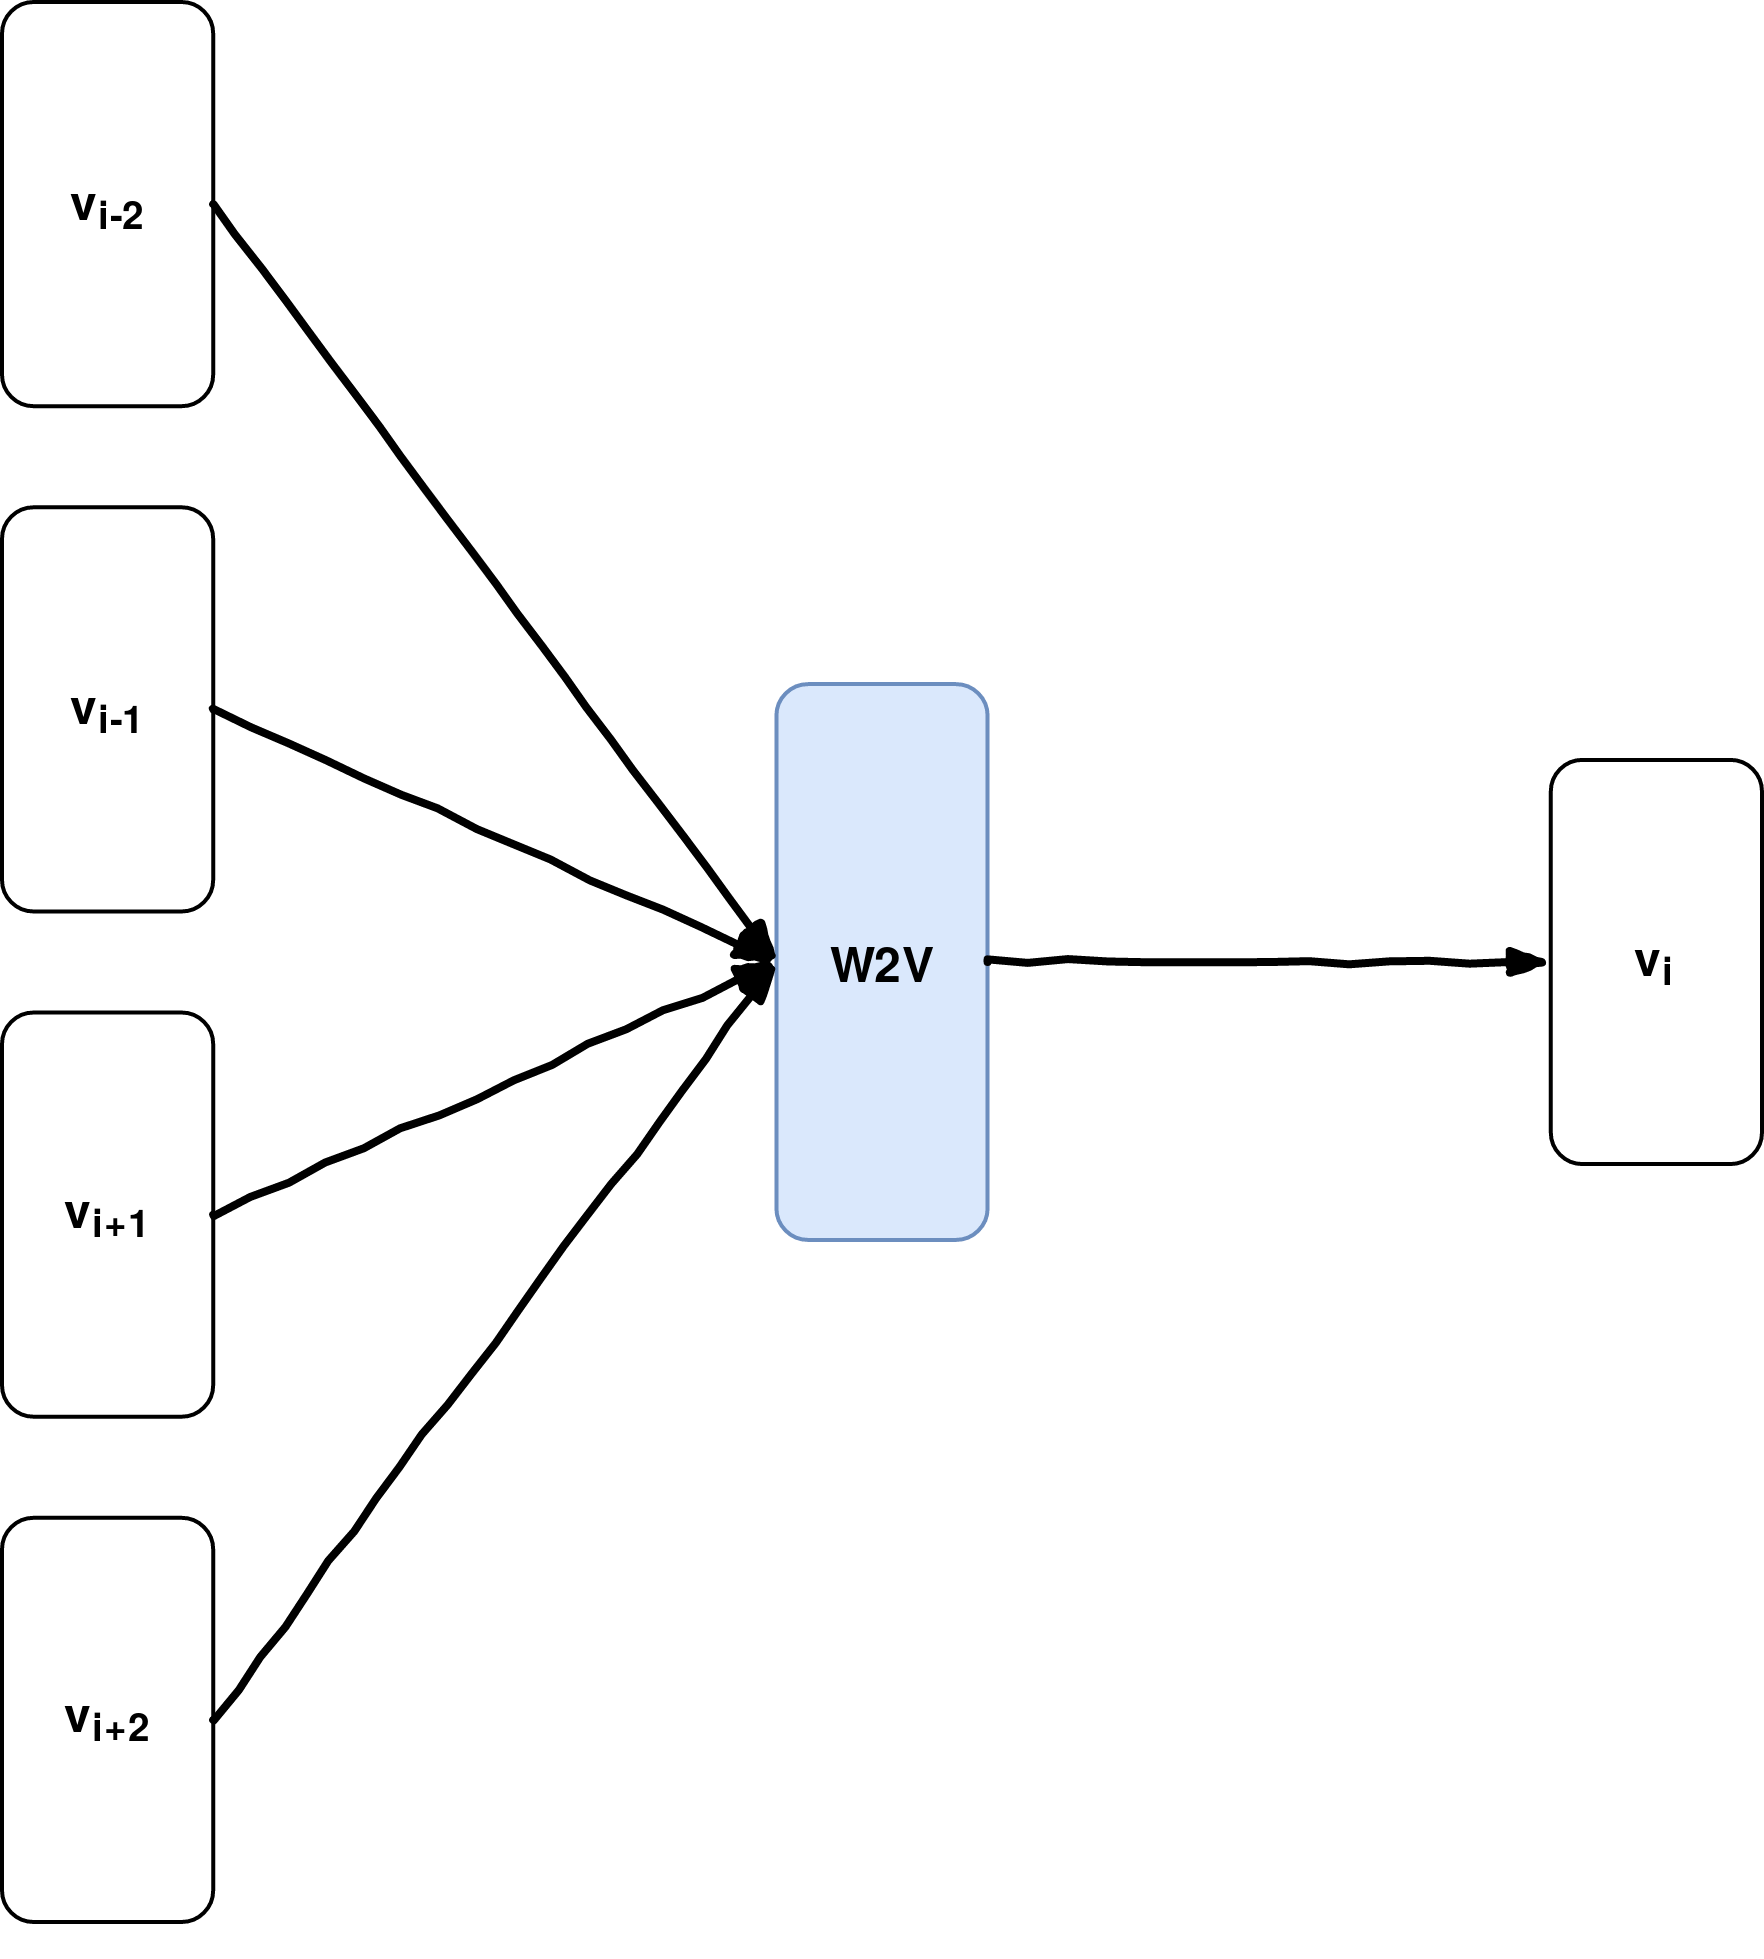
\includegraphics[width=0.5\textwidth,height=150px]{cbow}
	\caption{CBOW modell}
\end{figure}

Skip-Gram modell esetén pont az ellenkezője történik. A háló bemenete $v_i$
$\left( i \in \left|D\right| \right)$ vektor lesz. A tanítás célja, hogy a háló prediktálja az i. szó k méretű kontextusának one-hot kódolt vektorait ($v_{i-k},...,v_{i-1}, v_{i+1},..., v_{i+k} : k \in \mathbb{N}$), közben a háló a rejtett rétegében megtanulja a Word2Vec reprezentációt.

\begin{figure}[H]
	\centering
	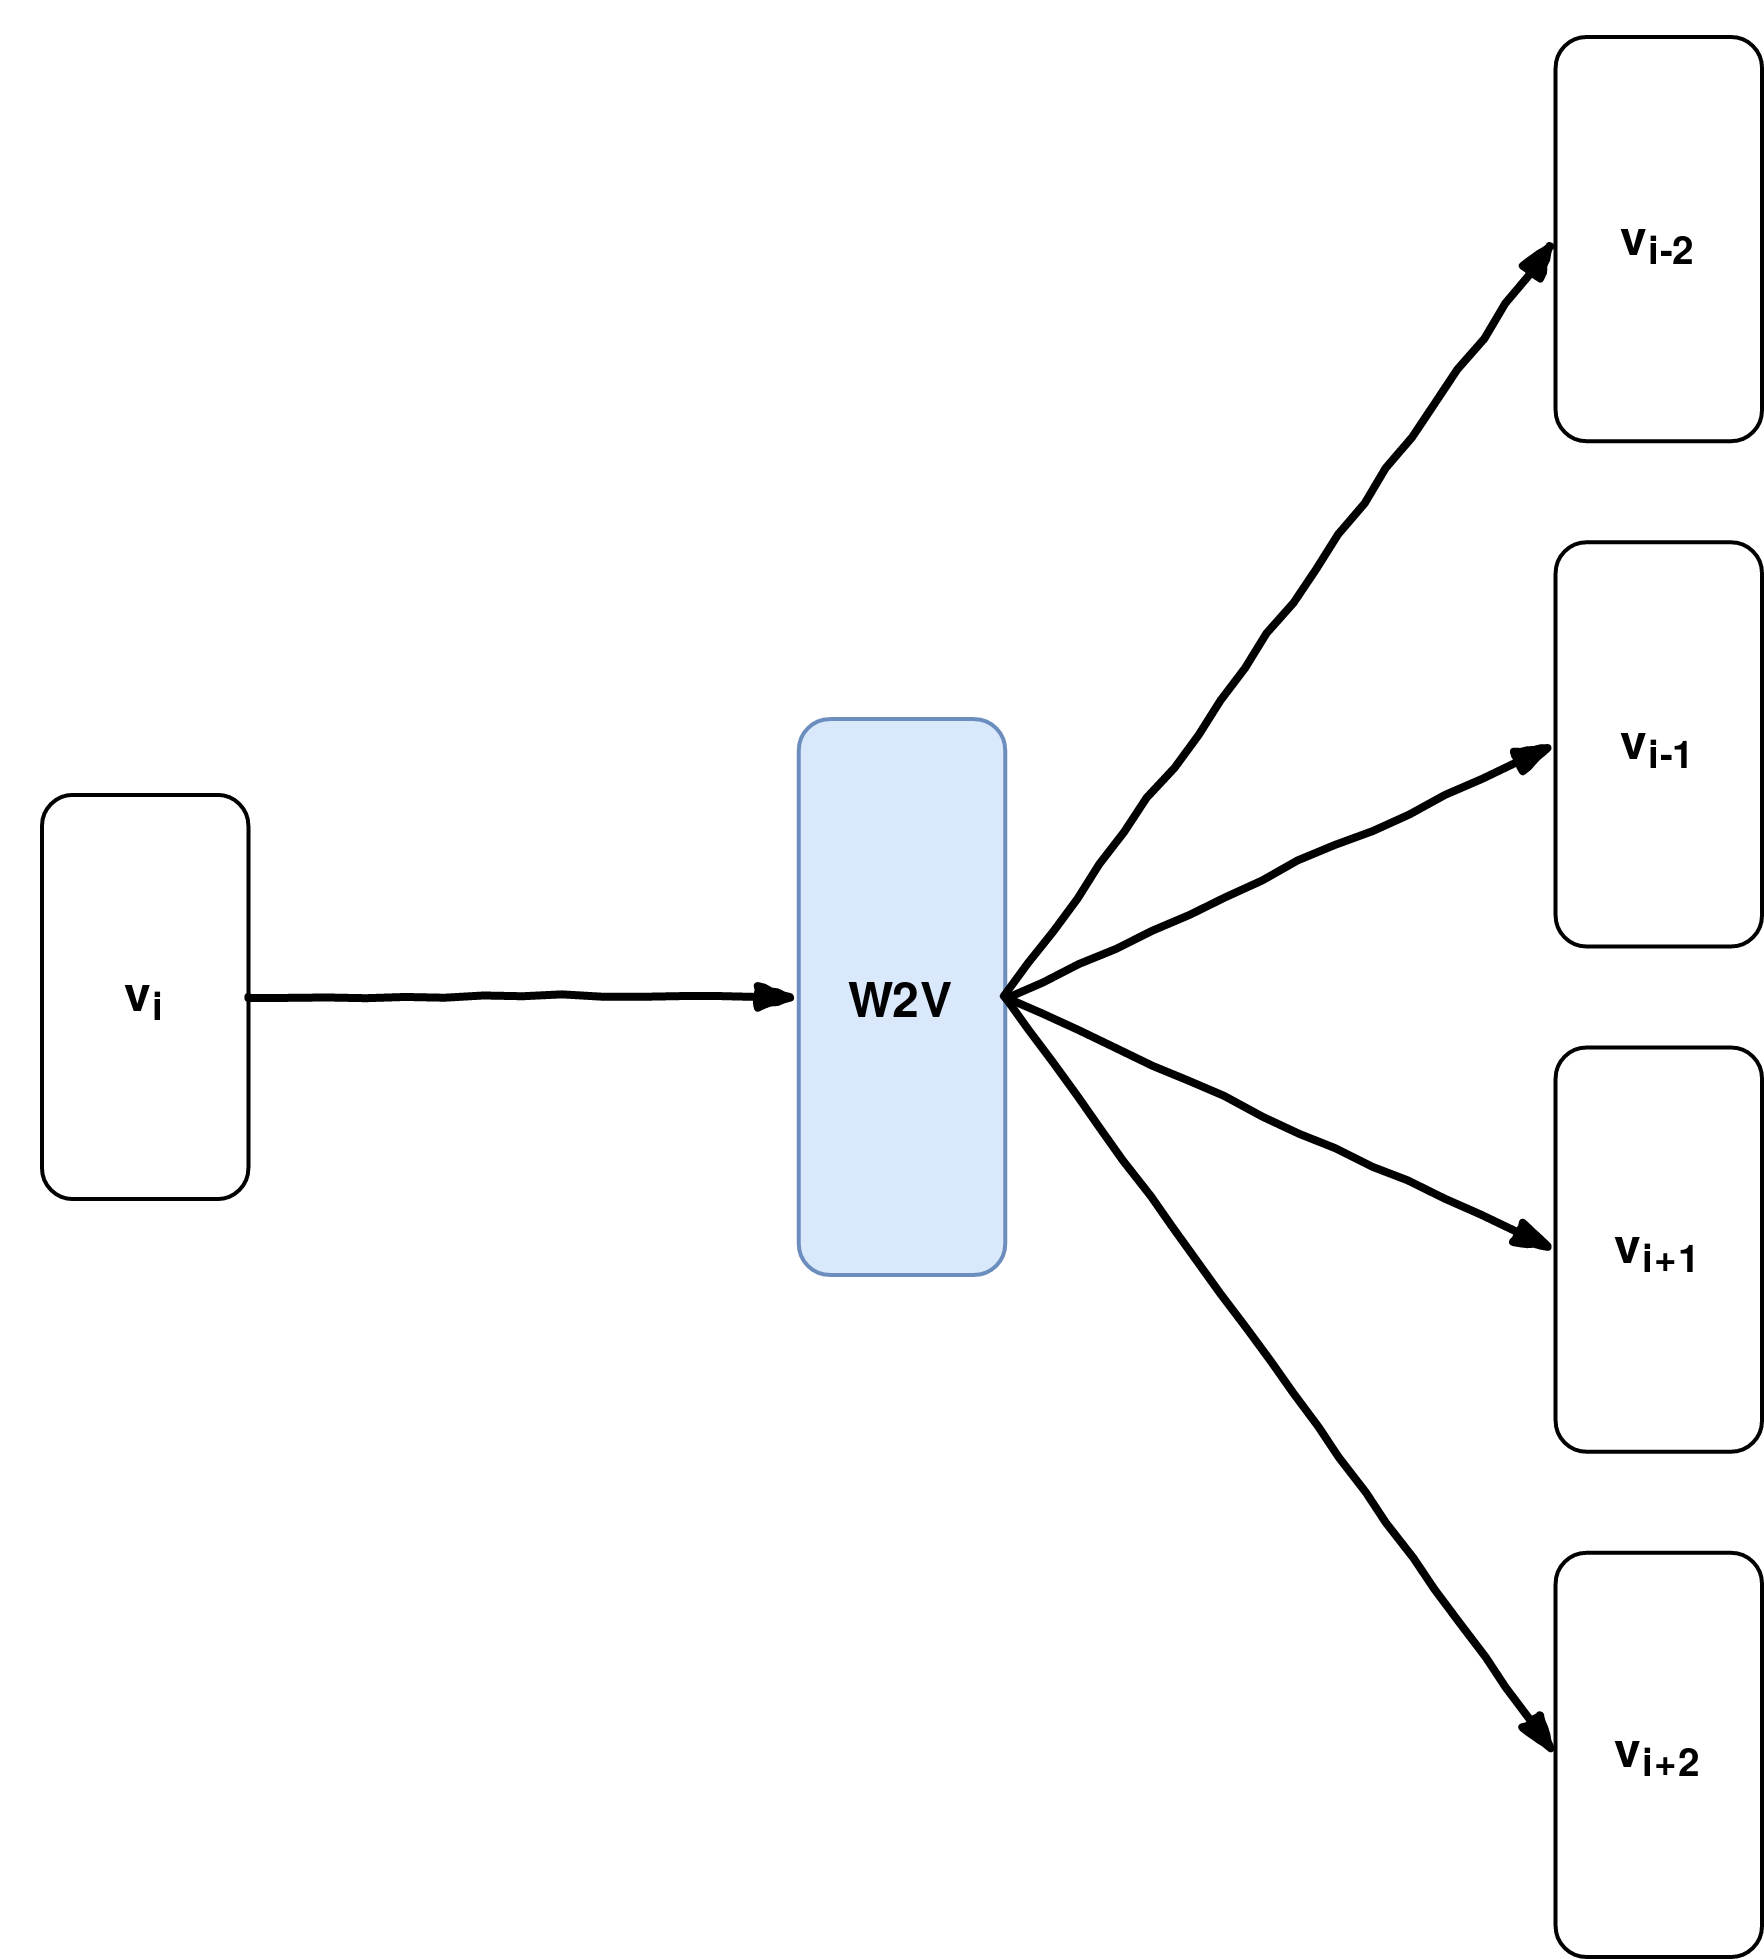
\includegraphics[width=0.5\textwidth,height=150px]{skip-gram}
	\caption{Skip-Gram modell}
\end{figure}

\begin{note}
	A Skip-Gram modell a ritka szavak, míg a CBOW modell a gyakori szavak esetén készít pontosabb reprezentációt.
\end{note}


\subsubsection{GloVe}
A GloVe (Global Vectors) reprezentációs módszer egy korpusz lokális statisztkáján kívül a globális statisztikáit is figyelembe veszi. 

\begin{definition}
	Adott egy korpusz, melynek elemszáma V. Az $X \in \mathbb{N}^{V \times V}$ mátrixot közös előfordulási mátrixnak nevezzük, ahol $X_{ij}$ az a szám, ahányszor i. szó kontextusában j. szó megjelenik.  
\end{definition}

A GloVe modell tanítása egy korpusz közös előfordulási mátrixának nem nulla elemein történik. A GloVe modell egy log-bilineáris modell, amely feladata, hogy kiszámítsa a következő szó valószínűségét azon kontextusa alapján.

A módszer mögötti intuíció az, hogy a közös előfordulási valószínűségek hányadosa értékes információval szolgálhat a leképezés során. Így a feladat célja, hogy a tanult szóvektorok skaláris szorzata megegyezzen a szavak közös előfordulási valószínűségének logaritmusával. Mivel $\log \left( \frac{A}{B} \right) = \log \left( A \right) - \log \left( B \right)$, így ez a cél összekapcsolja az előfordulási valószínűségek arányszámát a vektorok távolságával.

\begin{note}
	A GloVe módszer néhány esetben túlteljesíti a Word2Vec-et.
\end{note}

\subsubsection{ELMo}
A Word2Vec és a GloVe csak szavankénti kontextusfüggetlen reprezentáció tanulására képes. Az Embeddings from Language Models (ELMo) módszer figyelembe veszi azon szó kontextusát is, amelyre éppen alkalmazzák. Az ELMo használat közben állítja elő a vektorokat.

A modell tanításához használt neurális háló több réteg kétirányú LSTM (biLSTM) konkatenációja. A különböző rétegek más és más típusú információt képesek eltárolni.

\begin{figure}[H]
	\centering
	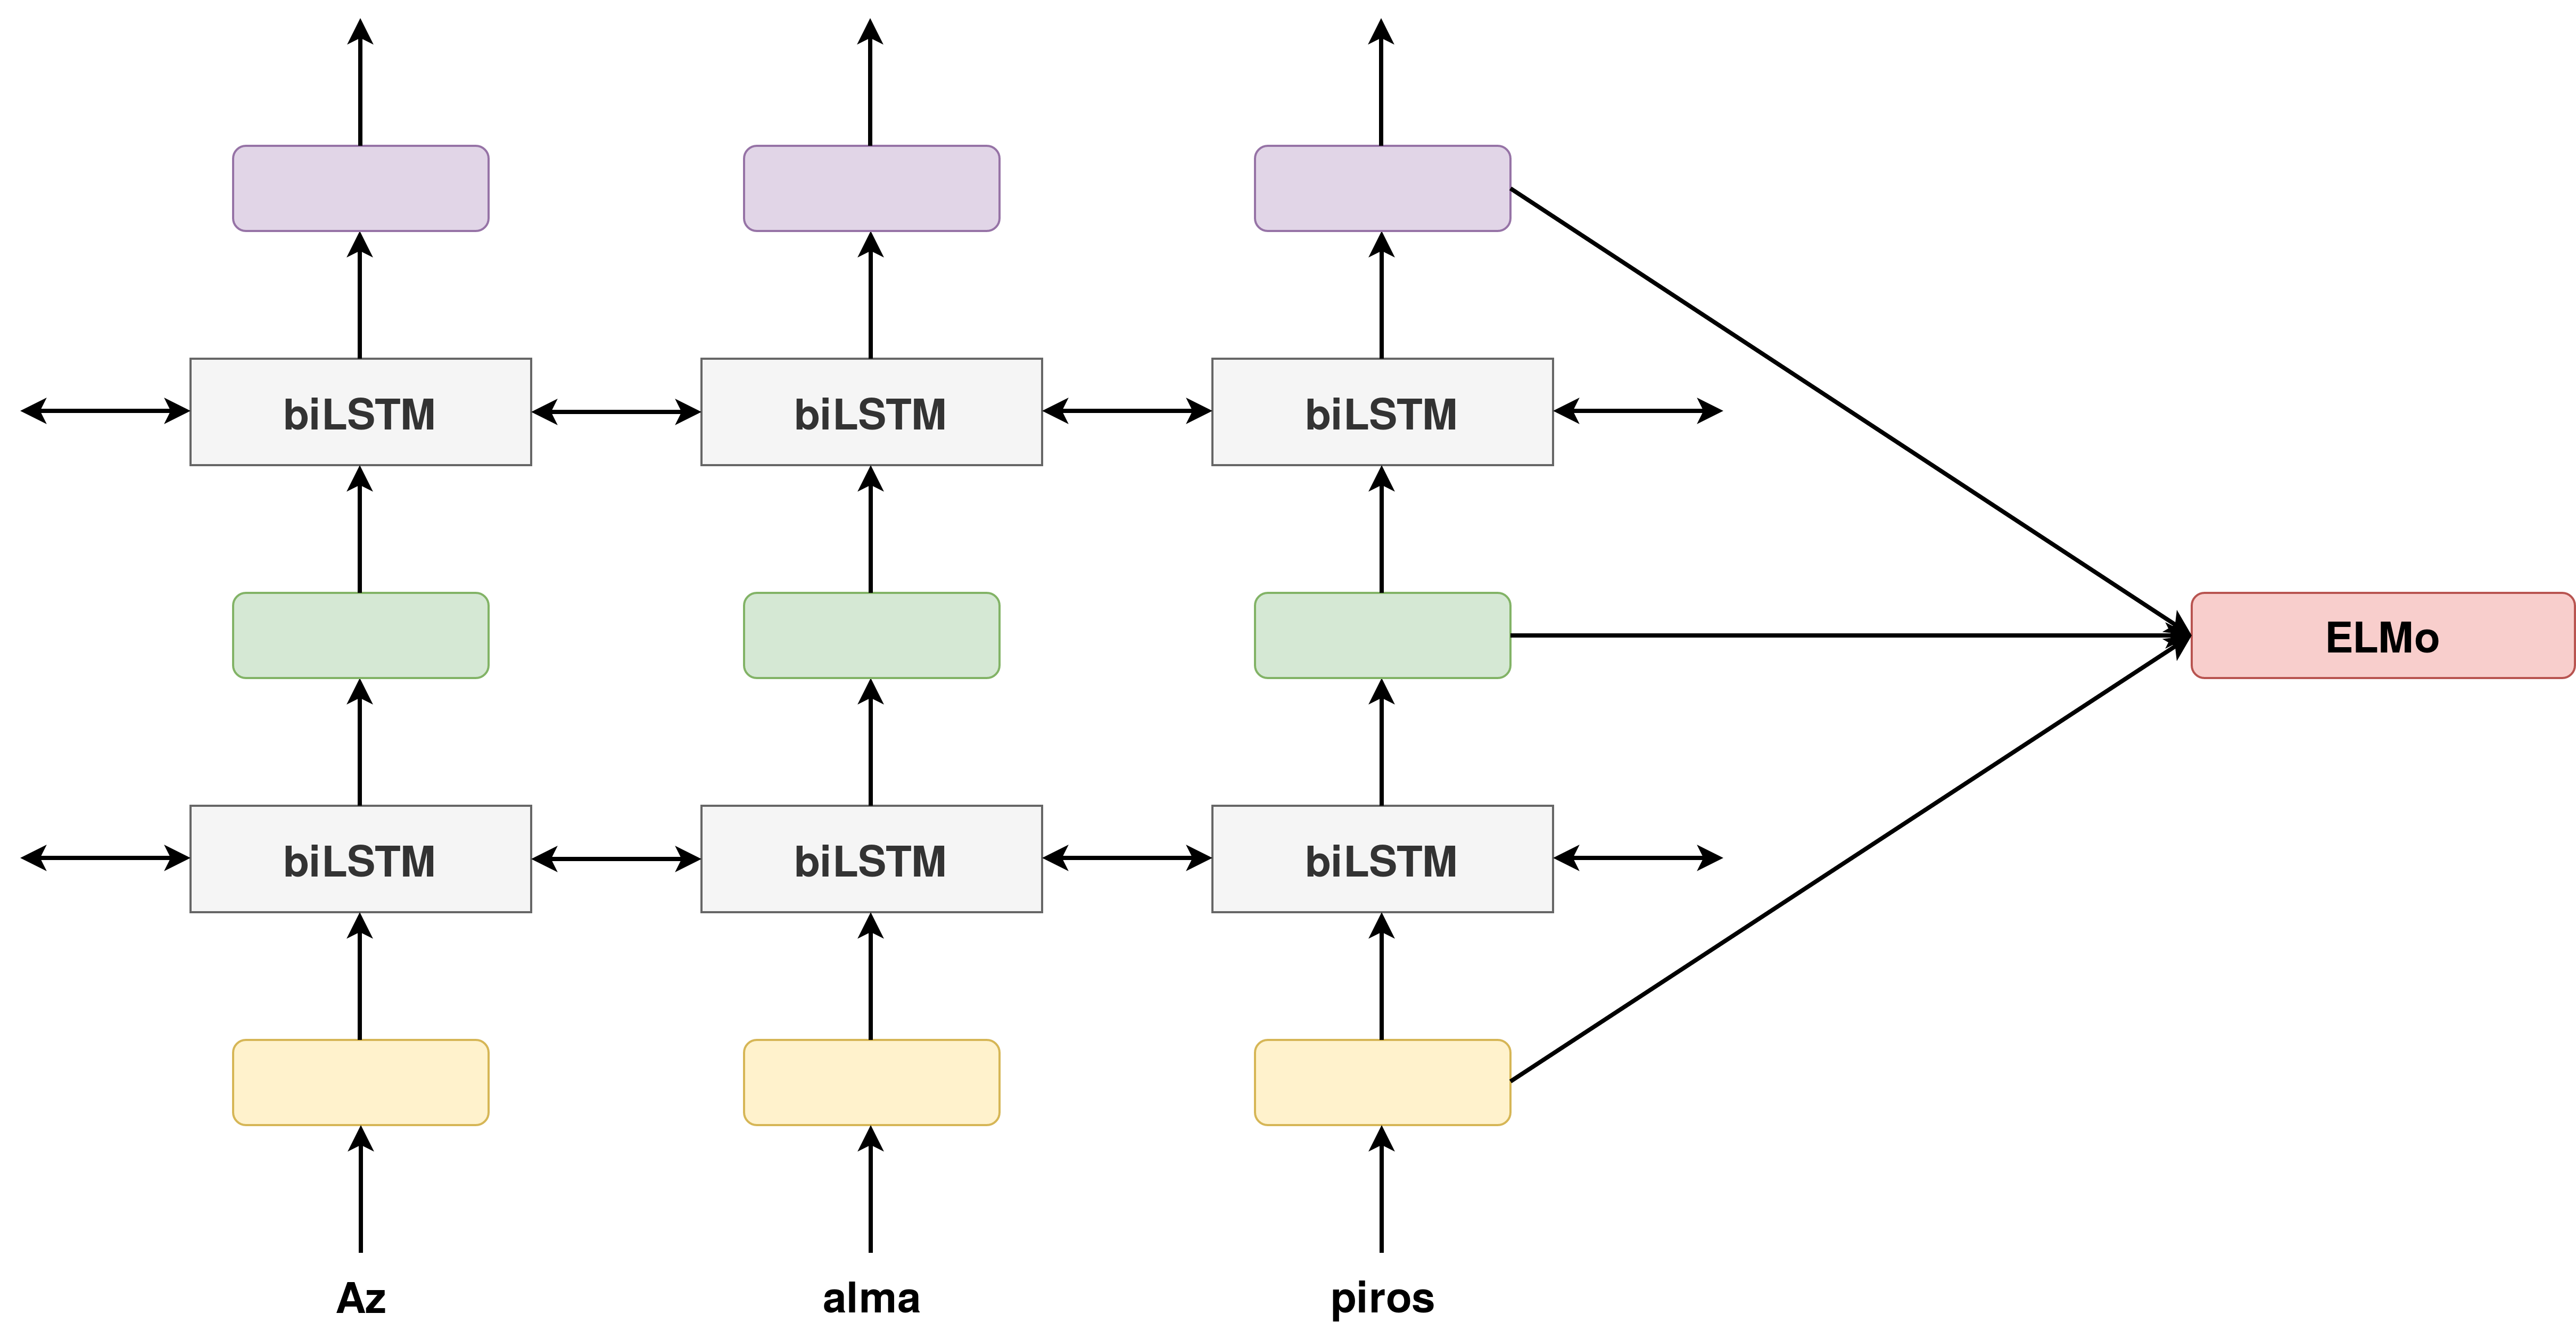
\includegraphics[width=0.8\textwidth,height=200px]{ELMo}
	\caption{ELMo modell}
\end{figure}

Az ELMo a különböző rétegek kimenetének feladatspecifikus kombinációján alapszik. Egy adott NLP feladatra minden biLSTM réteg egyedi súlyt kap. A végső háló 2 darab biLSTM rétegből áll, minden LSTM réteg 4096 széles.

Az így kapott sekély kétirányú módszer jelentősen javított a szóvektorok pontosságán.

\begin{note}
	Az ELMo egy karakter alapú reprezentációs módszer, így képes kezelni az addig nem látott szavak problémáját is.
\end{note}

\subsubsection{BERT}
A Bidirectional Encoder Representations from Transformers (BERT) egy a Google által kifejlesztett transformer architektúrájú nyelvi modell. Az ELMo-hoz hasonlóan ez is kétirányú, azaz egy szó mindkét oldali kontextusát figyelembe veszi a tanulás alatt. 

A tanítást két fázisra bontották: előtanítás és finomhangolás.

Az előtanítás két feladatból állt: \textit{következő mondat} és \textit{maszkolás}. A \textit{következő mondat} esetében a mélyháló feladata kitalálni, hogy A[SEP]B input mondatokra B rákövetkezője-e A-nak. A \textit{maszkolás} során véletlenszerűen letakarták a szavakat a mondatokban és a mélyháló megpróbálta kitalálni, hogy eredetileg melyik szó volt a [MASK] token helyén.

\begin{figure}[H]
	\centering
	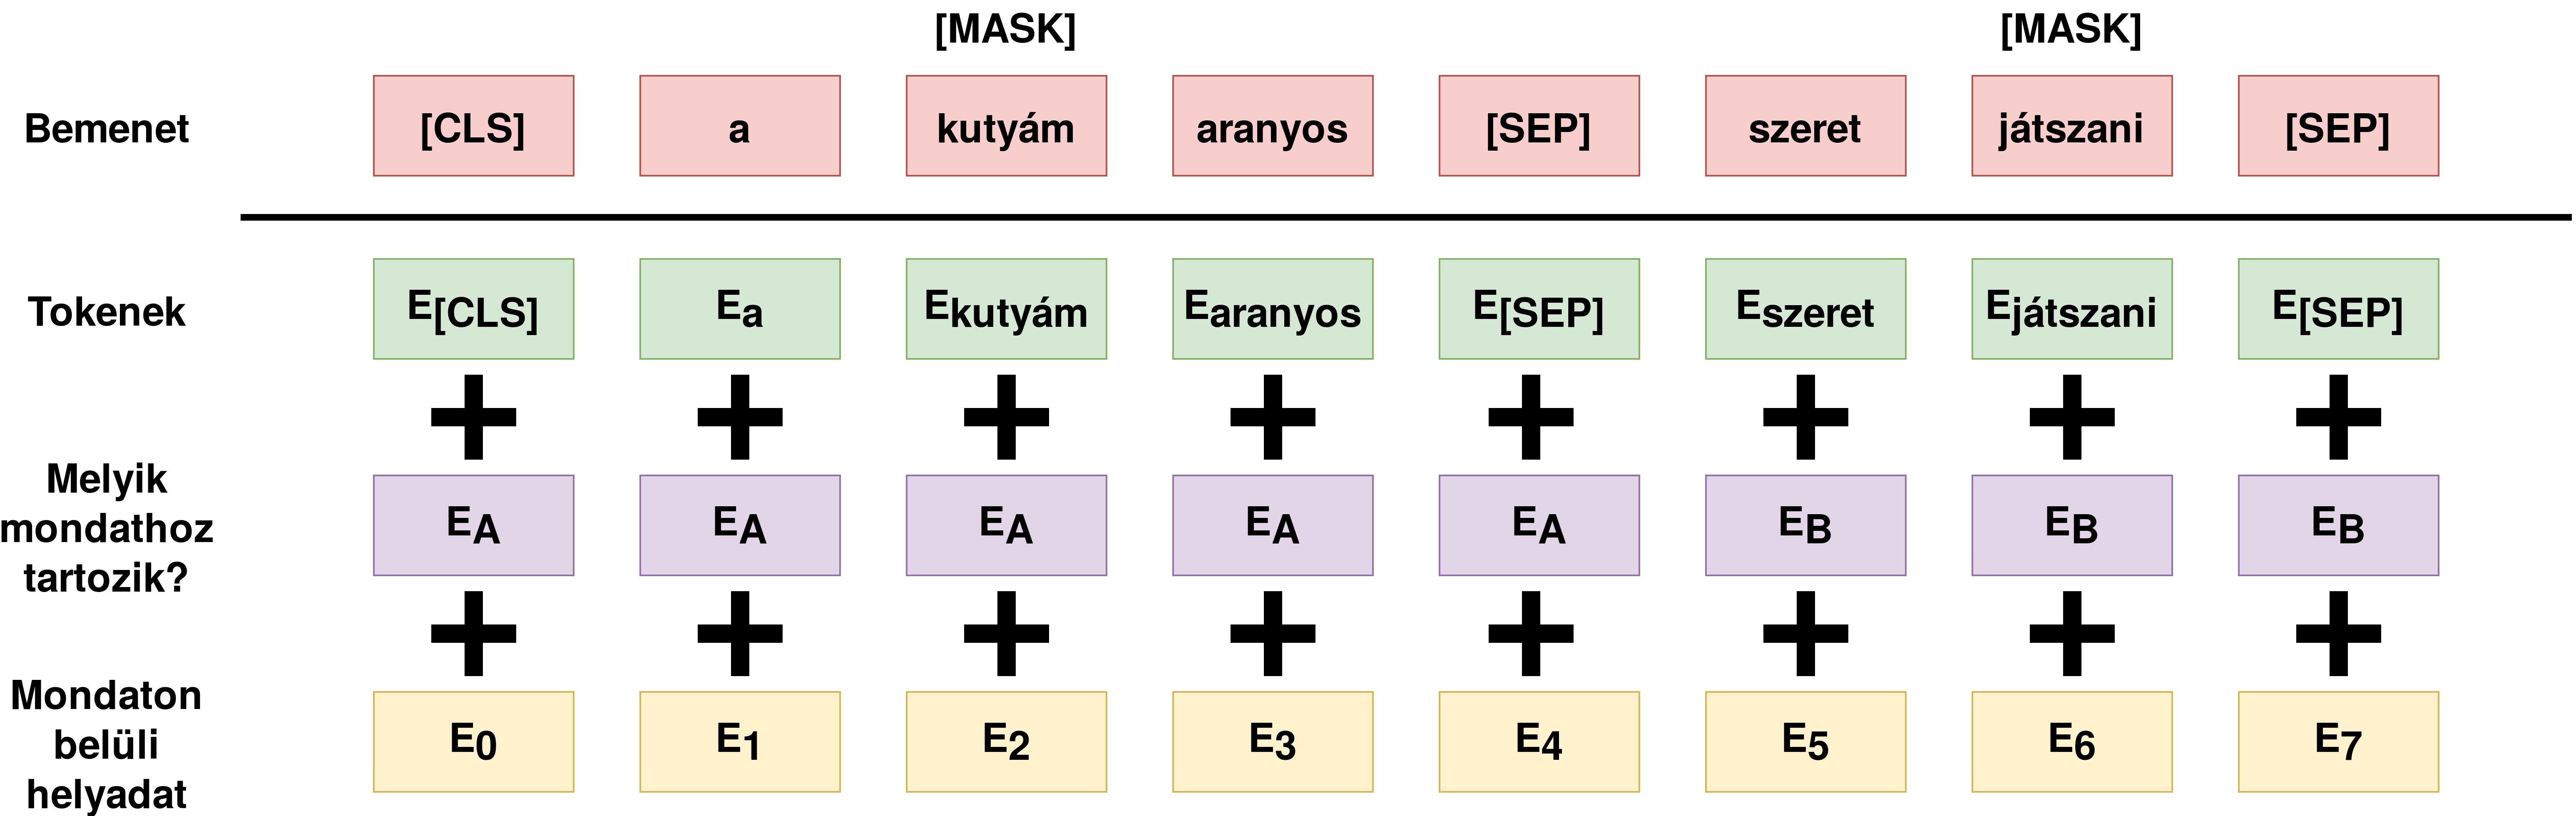
\includegraphics[width=1\textwidth,height=160px]{BERT}
	\caption{A BERT bemenete}
\end{figure}

A bemenetben megadták a token-eket, a token-ekhez tartozó mondaton belüli helyadatokat és azt, hogy az adott token A vagy B mondathoz tartozik.


A finomhangolás az adott NLP feladat szerint történik.

\begin{note}
	Míg az ELMo különböző balról-jobbra és jobbról-balra olvasó rétegek konkatenációjaként állítja elő a reprezentációkat, addig a BERT a valódi mély architektúrájával csak egyszer dolgozza fel a token-eket. Több feladat megoldásában is jelenleg a BERT a State-of-the-art.
\end{note}



\section{Reprezentáció a mondatok és magasabb nyelvi elemek szintjén}
Néhány NLP feladatnál, mint például a dokumentumok szemantikus keresésénél, vagy szöveg összegzésnél szükség lehet magasabb szintű reprezentációkra. Ezek a módszerek szavak helyett mondatokat, bekezdéseket, vagy akár egész dokumentumokat tesznek numerikusan értelmezhetővé. 

\subsection{Mondatvektorok}
A szóvektorokhoz hasonlóan mondatvektorokat úgy kapunk, ha mondatokat helyezünk el egy vektortérbe. A módszerünk akkor hatékony, ha az azonos jelentéstartalmú mondatok reprezentációi klaszterekbe tömörülnek a vektortérben.


\subsubsection{Skip-thought vektorok}
A Skip-though módszer a Skip-Gram algoritmus mondatokra történő kiterjesztése. A szerzők rekurrens enkóder-dekóder hálót használtak a tanításhoz, melynek bemenete mondathármasok Word2Vec vektoraiból állt. A háló feladata $s_i$ mondat esetén $s_{i-1}$ és $s_{i+1}$ mondatok generálása volt.

\begin{figure}[H]
	\centering
	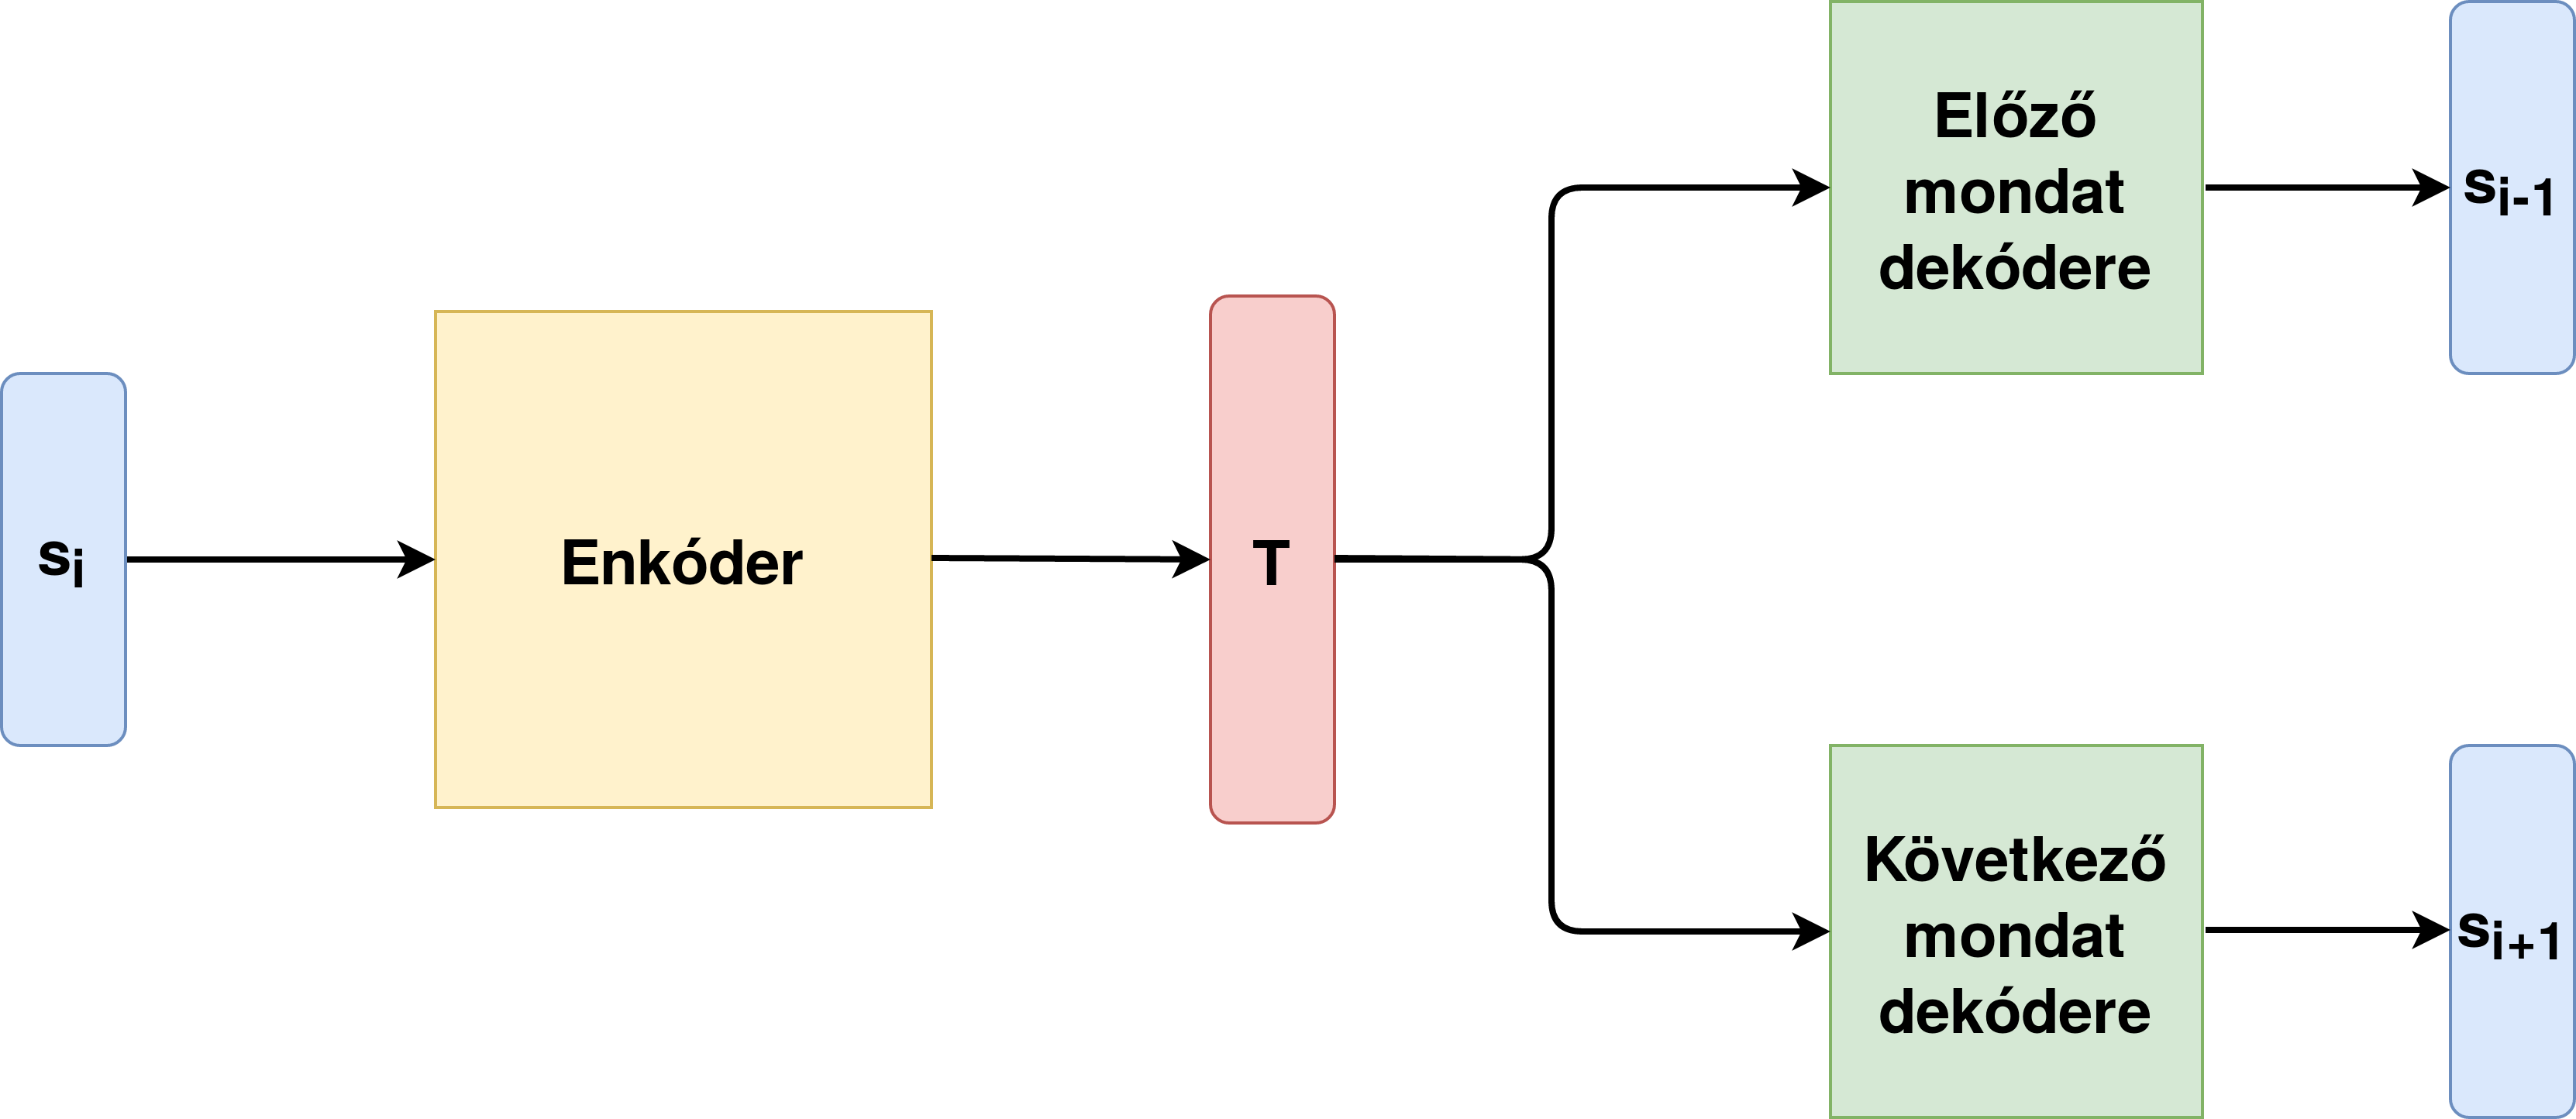
\includegraphics[width=0.6\textwidth,height=130px]{Skip-thought}
	\caption{A Skip-thought enkóder-dekóder arcitektúrája}
\end{figure}

A rekurrens modell GRU aktivációkkal bírt.
Olyan szavak esetén, melyeket a háló még nem ismert, tanítottak egy $f:V_{w2v} \rightarrow V_{rnn}$ lineáris leképezést, ahol $V_{w2v}$ és $V_{rnn}$ rendre a Word2Vec és a rekurrens GRU modell szótára. A reprezentáció vektora a rejtett, úgy nevezett \textit{thought} vektor (T).

\subsubsection{USE}
A Universal Sentence Encoder (USE) egy Google által fejlesztett mondatszintű szemantikus reprezentációs algoritmus. A szerzők két architektúrát használtak: a BERT-ben említett transformer-t és a DAN-t (Deep Averaging Network). 

\begin{figure}[H]
	\centering
	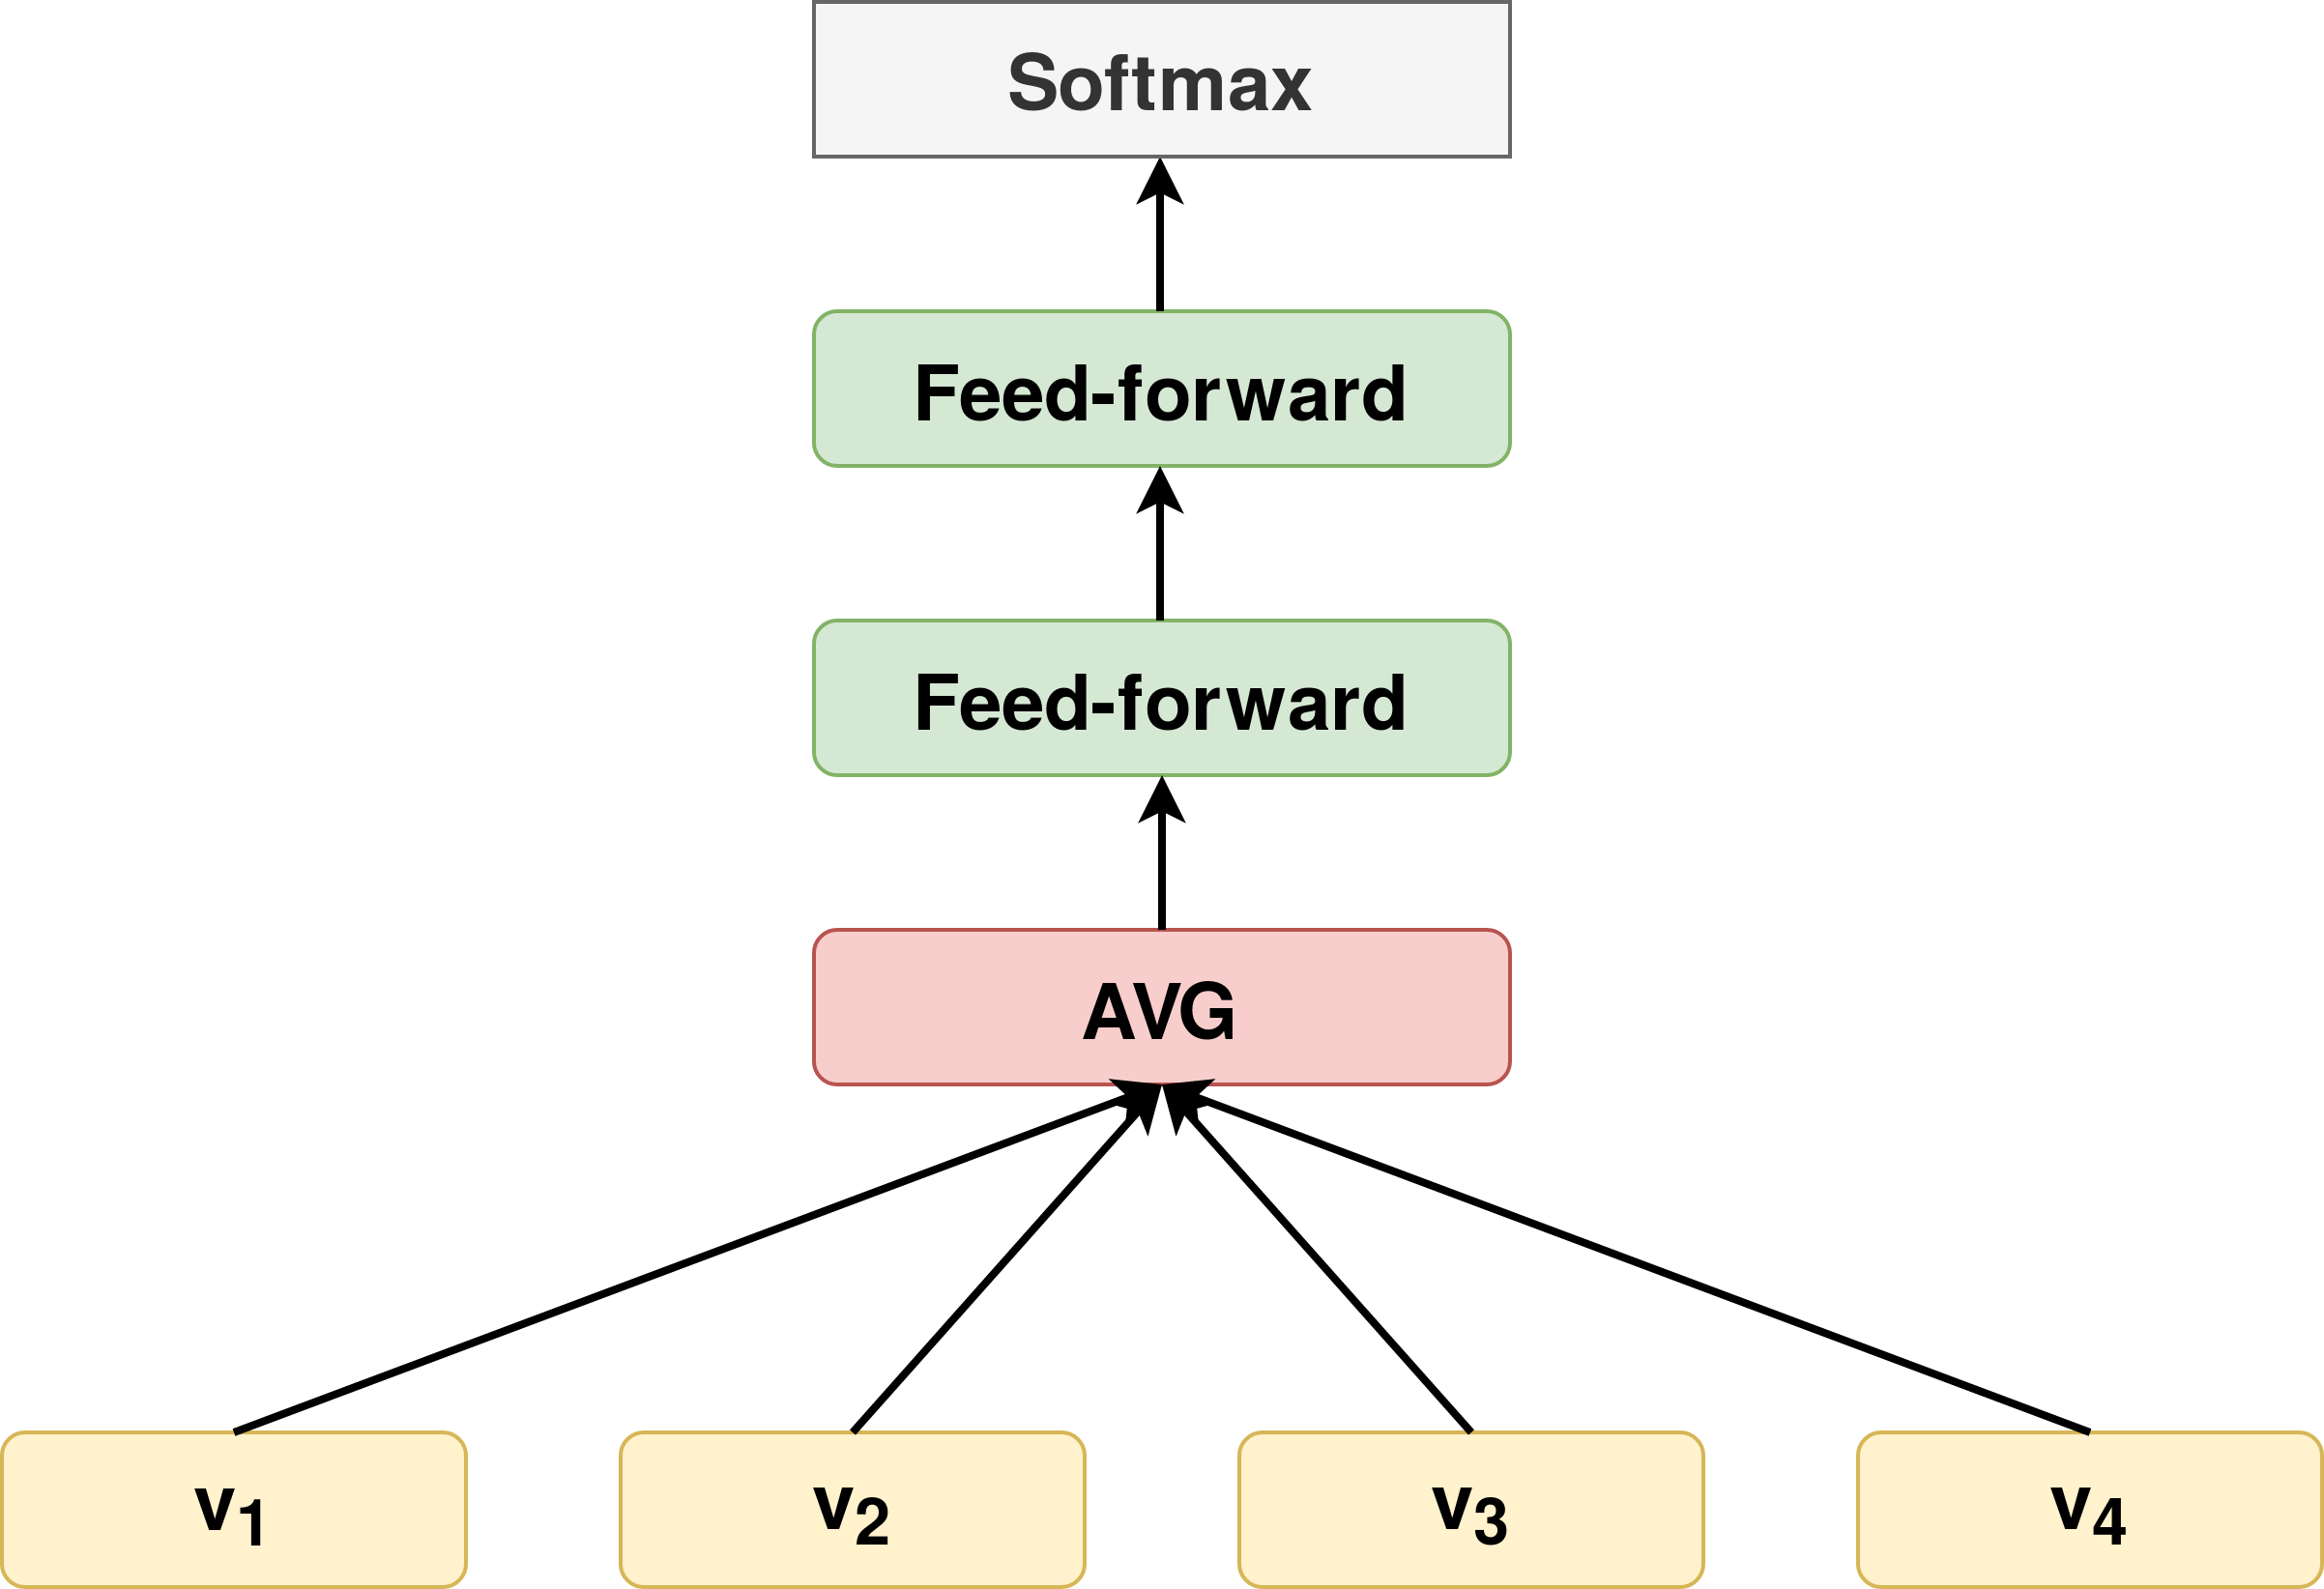
\includegraphics[width=0.6\textwidth,height=150px]{DAN}
	\caption{DAN architektúra}
\end{figure}

A hálókat (az ELMo-ban és a BERT-ben is bemutatott) transfer learning módszerrel tanították. A tanulás a Skip-thought-hoz hasonló módon és társalgásból vett mondat-válasz párokkal, illetve felügyelt módon a Stanford Natural Language Inference (SNLI) korpuszon történt.

A USE szavakból, mondatokból, vagy akár rövidebb bekezdésekből is képes 512 méretű vektorokat generálni.

A transformer modell pontosabb eredményt hozott, mint a DAN alapú modell, de a transformer modell $\mathcal{O}(n^2)$, míg a DAN modell $\mathcal{O}(n)$ időkomplexitású a bemeneti hossz függvényében. Továbbá memóriahasználatban is kedvezőbb választás a DAN háló.

\subsubsection{InferSent}
Az InferSent egy mondatszintű szemantikus reprezentációs technika, melyet a Facebook prezentált. Hasonló algoritmusokkal ellentétben a szerzők felügyelt tanítást végeztek, melyhez az SNLI adathalmazt vették igénybe.

Az SNLI adathalmaz 570 ezer darab – ember által írt és címkézett – mondatpárból áll. A címkék a következők: következmény, ellentmondás és semleges.

Négy háló architektúrát összemérve a legpontosabb eredményt a biLSTM + max pooling mutatta. 

\begin{figure}[H]
	\centering
	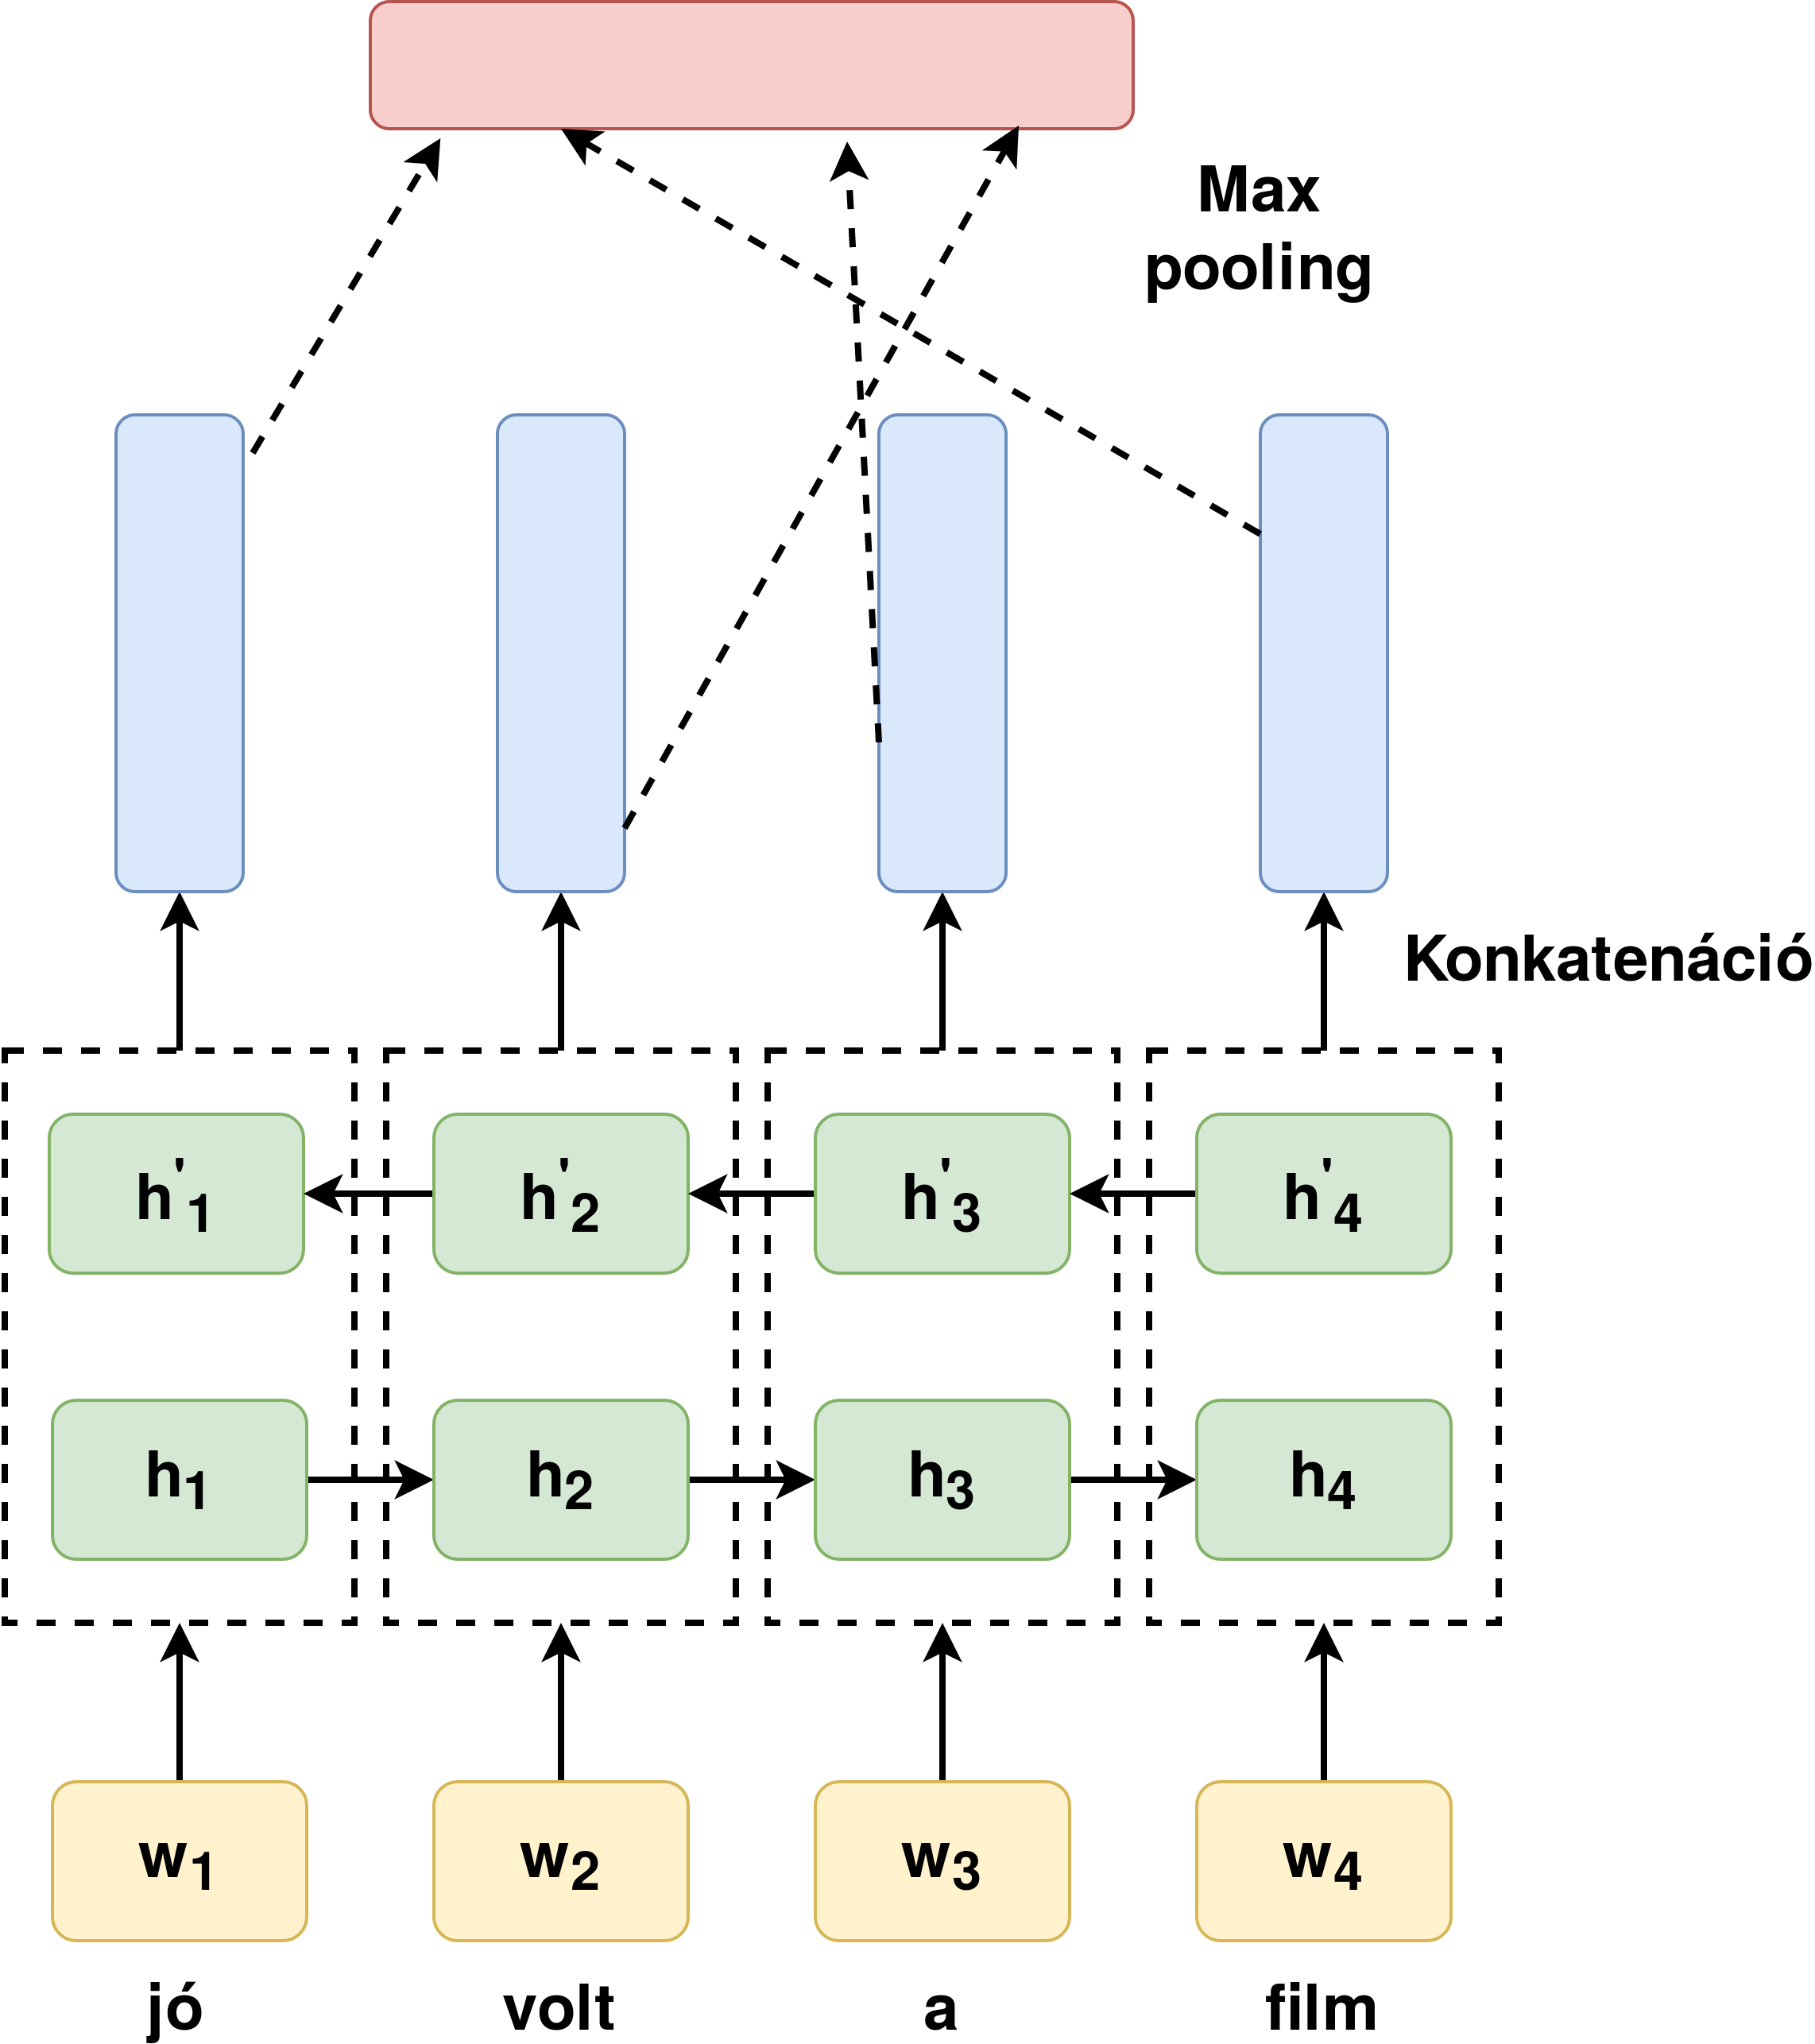
\includegraphics[width=0.5\textwidth,height=200px]{biLSTM-max-pooling}
	\caption{A biLSTM + max pooling architektúra}
\end{figure}

Az NLI feladat speciális szerkezetet igényel. Mivel kontextus független reprezentációt akartak előállítani, a mondatpárok GloVe vektorait szeparáltan enkódolták.

\begin{figure}[H]
	\centering
	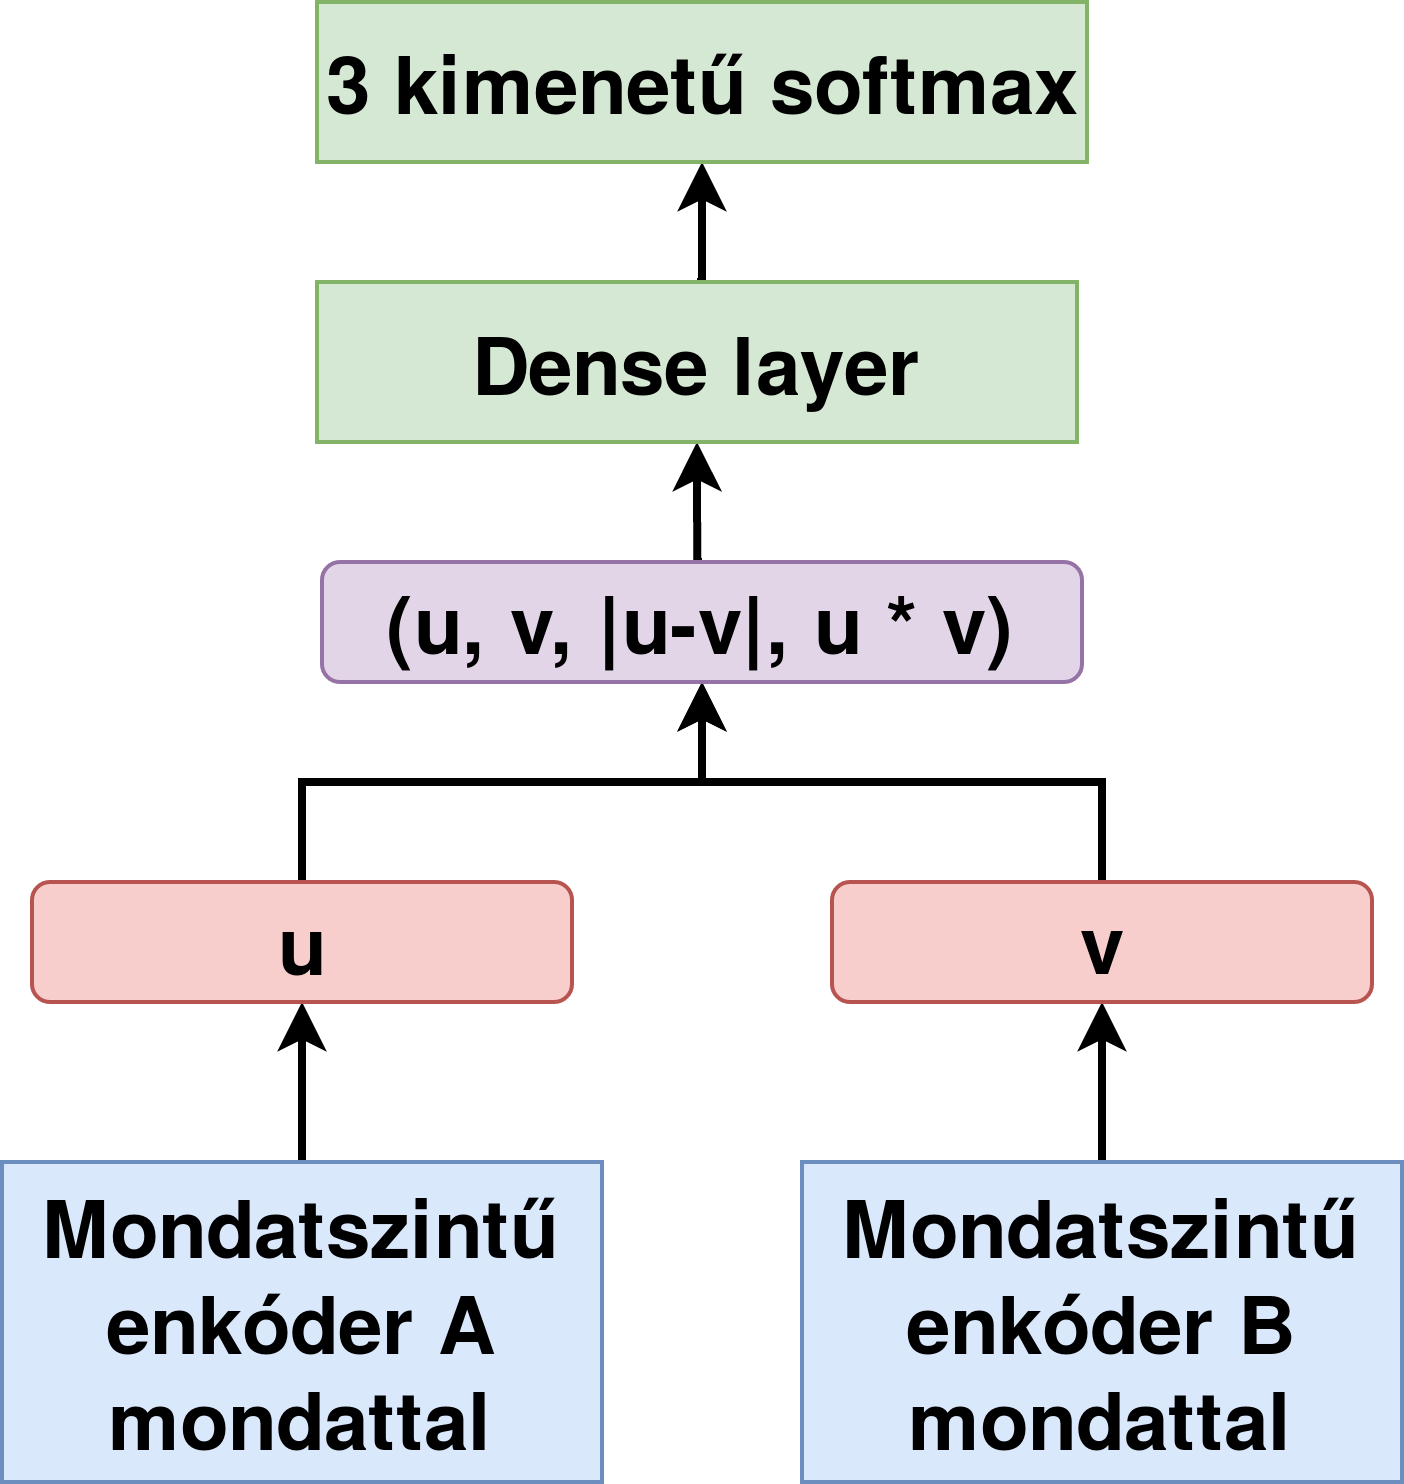
\includegraphics[width=0.5\textwidth,height=150px]{NLI}
	\caption{Az NLI feladat}
\end{figure}

Az így készült u és v vektorokból egy speciális reprezentáció készült: u, v, $\left| u - v \right|$ és $u \ast v$ (vektoriális szorzat) konkatenációjával, melyet végül egy 3 osztályú klasszifikáló hálóba vezettek.

\begin{note}
	A szerzők a reprezentációs vektorméret növelésével pontosabb eredményt kaptak.
\end{note}

\subsection{Doc2Vec}
A Doc2Vec módszer a Word2Vec modell kiterjesztése a dokumentumok szintjére. Mivel a dokumentumokat nem lehet a szavakhoz hasonló logikai struktúrába rendezni, ezért a megszokott CBOW modell bemeneti vektorai mellé egy speciális, a dokumentum azonosítóját jelölő vektort konkatenáltak. A tanítás végén a speciális vektor reprezentációja képviseli az egész dokumentumot.

\begin{figure}[H]
	\centering
	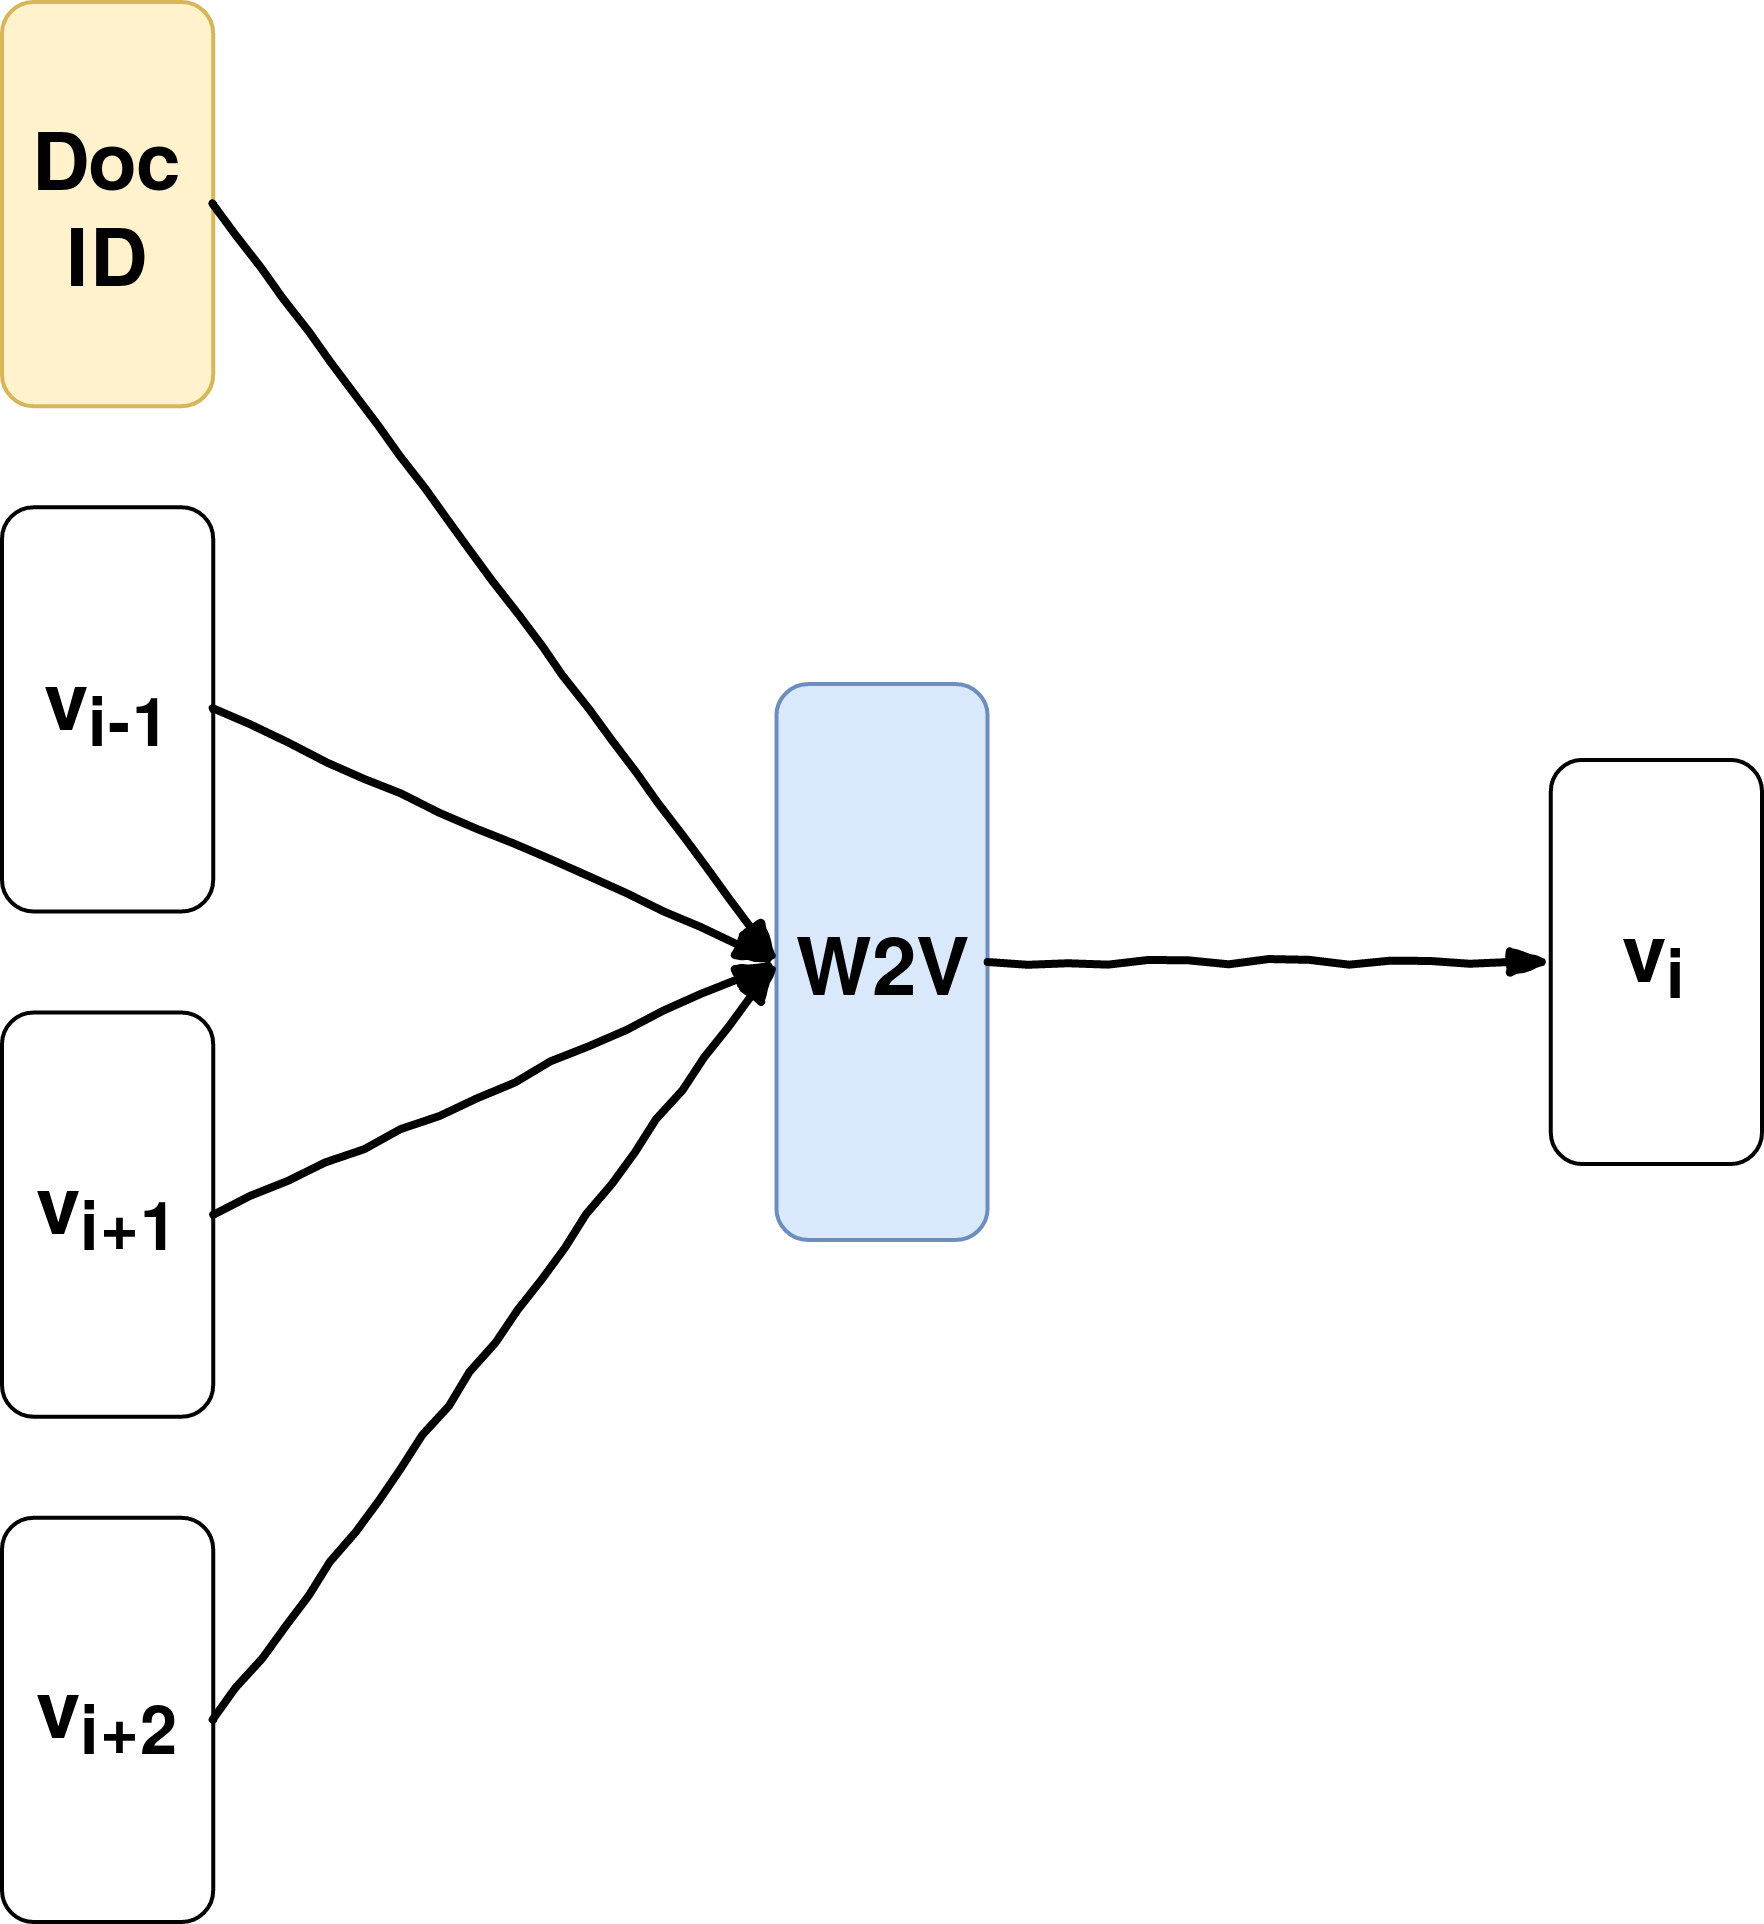
\includegraphics[width=0.5\textwidth,height=150px]{Doc2Vec}
	\caption{Doc2Vec PV-DM architektúra}
\end{figure}

Az így kapott modell képes dokumentumokat leképezni egy n dimenziós vektortérbe.

\section{Transfer learning}

A \textit{transfer learning} napjainkban közkedvelt tanítási módszer, melynek ötletét az NLP ágazata a számítógépes látás eszközkészletéből merítette. A folyamatot két fázisra lehet bontani: előtanítás és a finomhangolás. Az előtanítás általában nagy mennyiségű adaton történik. A finomhangolás az előtanítás után kapott modell – adott NLP feladathoz szükséges – speciális feladatokon való tanítását jelenti, ez szignifikánsan kevesebb adatot igényel.

\begin{definition}
	Jelölje $D_s$ a forrástartományt, $D_t$ a céltartományt, $T_s$ a forrástartományhoz tartozó feladatot, továbbá $X_t$ és $Y_t$ rendre a $T_t$ célfeladathoz tartozó inputváltozók és  címkék halmazát. A \textbf{transfer learning} célja megtanulni $P(Y_t|X_t)$ feltételes valószínűségi eloszlást $D_t$-ben $D_s$ által gyűjtött információ alapján úgy, hogy $D_s \neq D_t$ vagy $T_s \neq T_t$.	 
\end{definition}

\begin{figure}[H]
	\centering
	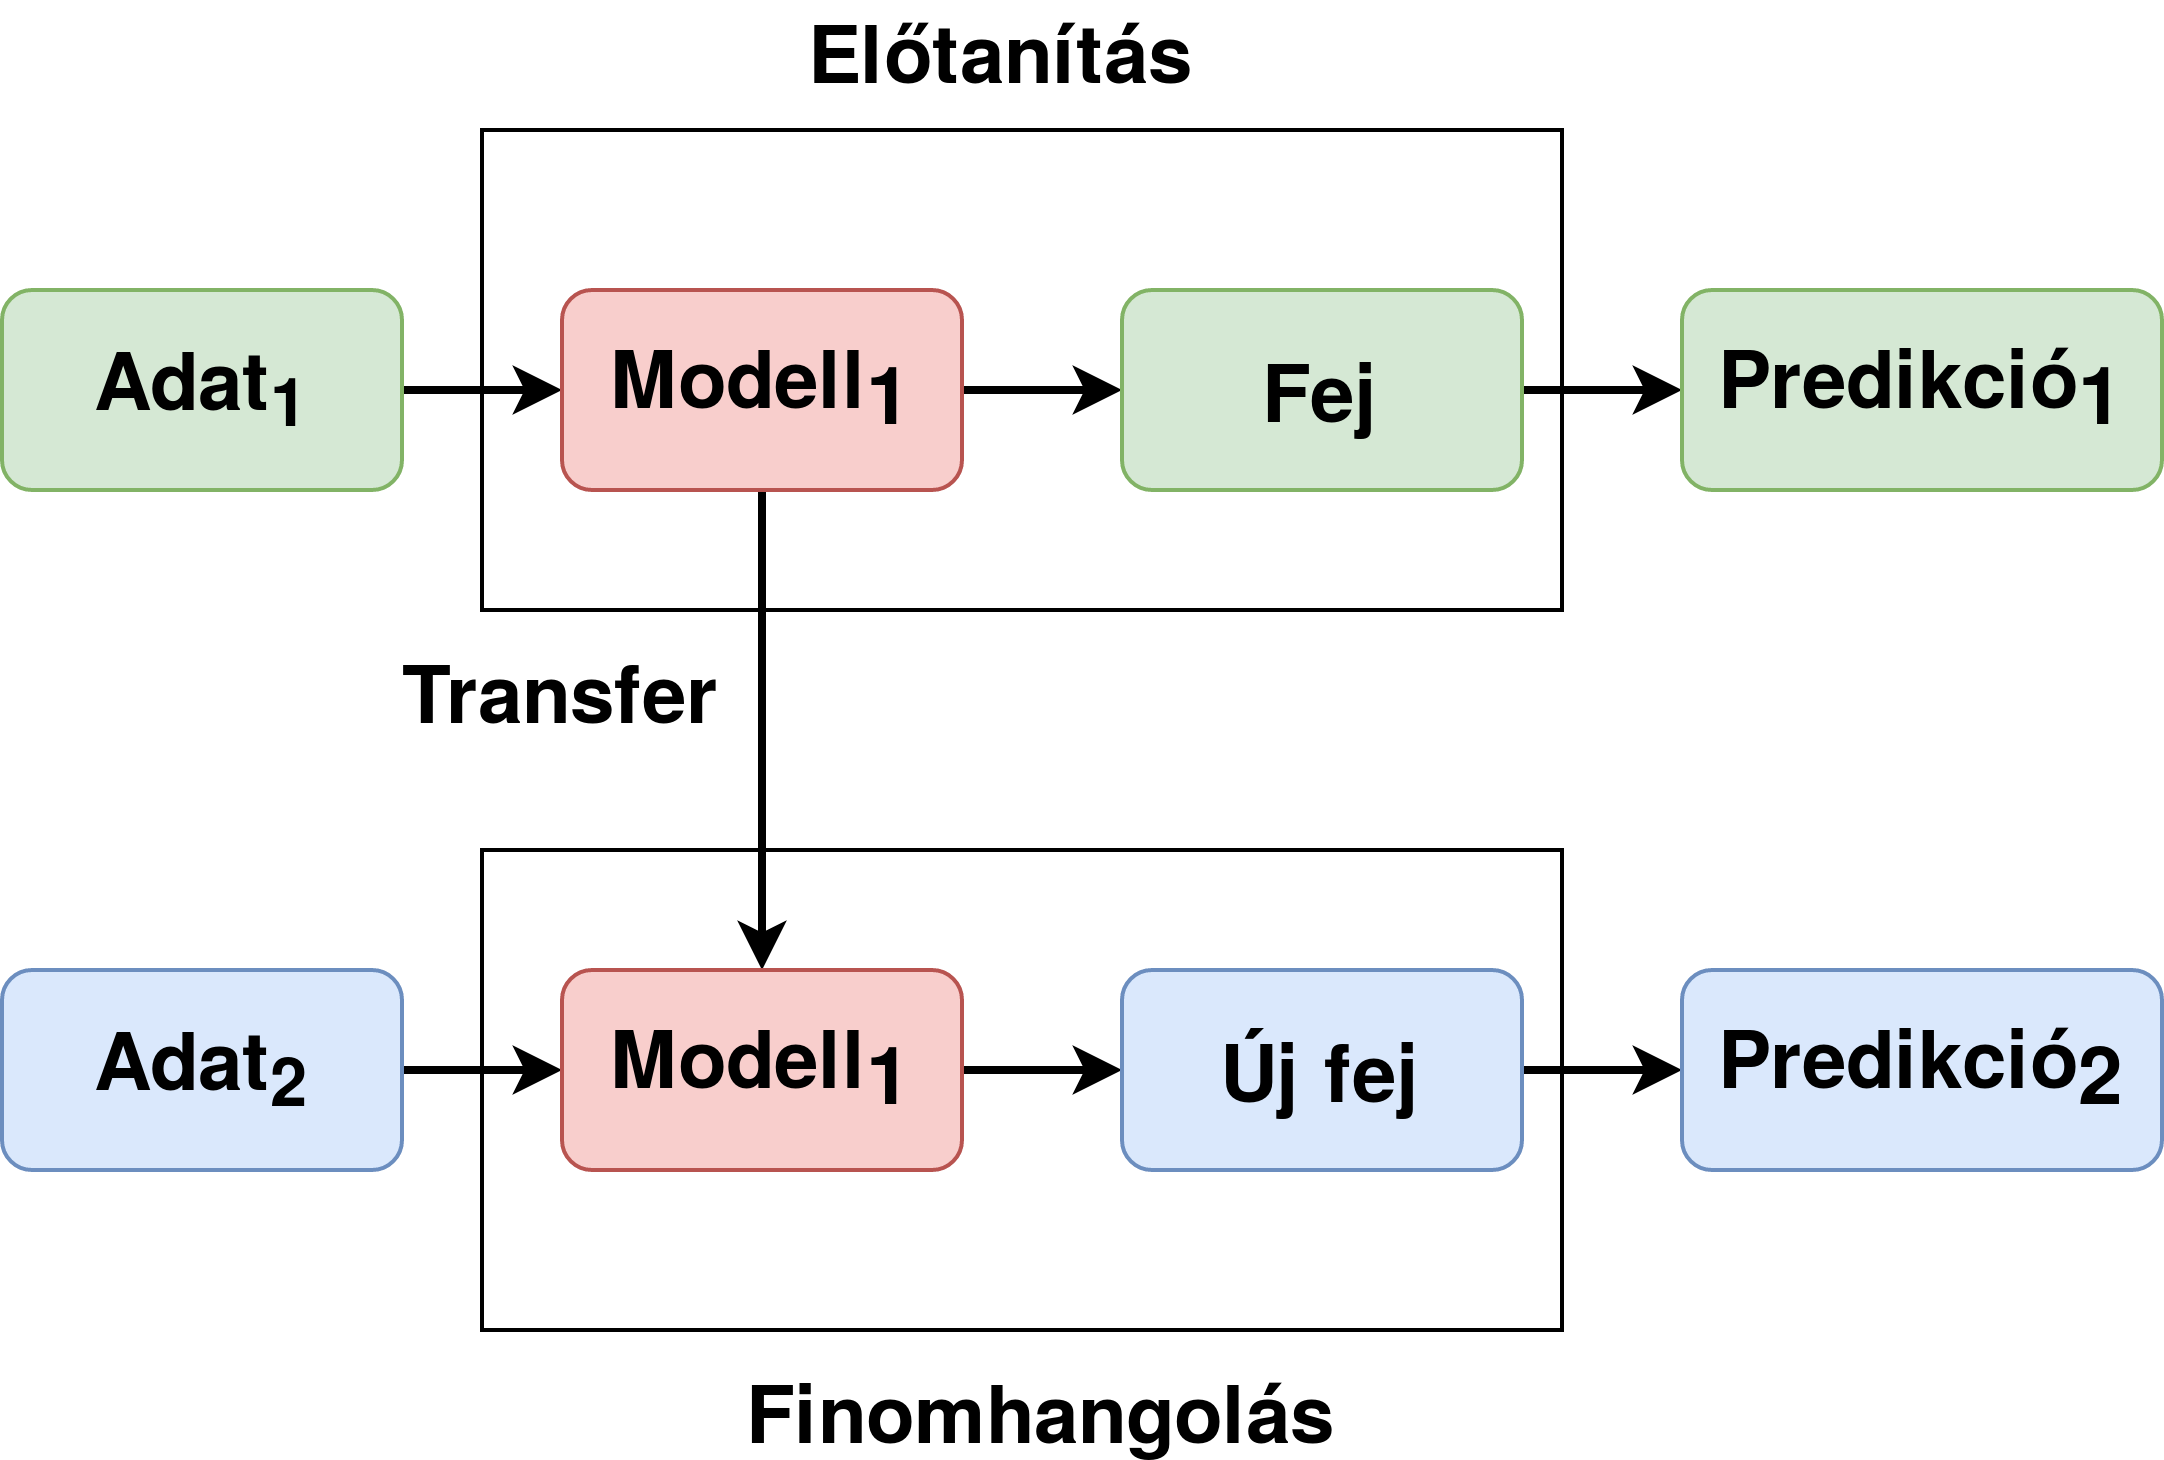
\includegraphics[width=0.6\textwidth,height=170px]{transfer}
	\caption{Transfel learning}
\end{figure}







